% RELIC - IEEEtran journal paper.
% Build: cd paper && mkdir -p build && nix run nixpkgs#tectonic -- main.tex -o build
% Numbers: run `.venv/bin/python paper/make_numbers.py` from the repository root. Every \N, \Pct
% and \CI key is a row of findings/results.csv, which names the pre-registration entry behind it.
\documentclass[journal,10pt]{IEEEtran}

\usepackage{booktabs}
\usepackage{amsmath}
\usepackage[T1]{fontenc}
\usepackage{newtxtext,newtxmath}
\usepackage{tikz}
\usetikzlibrary{arrows.meta,positioning,shapes.geometric,calc,backgrounds,fit}
\usepackage{graphicx}
\usepackage{xcolor}
\usepackage{array}
\usepackage{algorithm}
\usepackage{algpseudocode}
\usepackage[hidelinks]{hyperref}

\newtheorem{proposition}{Proposition}

% Abstract and index terms without the template's em dashes; no hyphenation in the index terms.
\makeatletter
\def\abstract{\normalfont\small\noindent\textbf{Abstract.}\enspace\@IEEEgobbleleadPARNLSP}
\def\IEEEkeywords{\normalfont\small\noindent\textbf{Index Terms.}\enspace
  \hyphenpenalty=10000\exhyphenpenalty=10000\@IEEEgobbleleadPARNLSP}
\makeatother

% Generated from results/live_learning/confirm/*_n1000_routed_eval.json (prereg SS64).
\newcommand{\cfEff}{0.997}
\newcommand{\cfEffPct}{99.7}
\newcommand{\cfEffCI}{.993,1}
\newcommand{\cfPara}{0.323}
\newcommand{\cfParaPct}{32.3}
\newcommand{\cfParaCI}{.295,.352}
\newcommand{\cfNoLeak}{0.992}
\newcommand{\cfNoLeakPct}{99.2}
\newcommand{\cfNoLeakCI}{.986,.997}
\newcommand{\cfGone}{0.96}
\newcommand{\cfGonePct}{96}
\newcommand{\cfGoneCI}{.92,.99}
\newcommand{\cfReturn}{0.96}
\newcommand{\cfReturnPct}{96}
\newcommand{\cfReturnCI}{.92,.99}
\newcommand{\cfRetain}{0.997}
\newcommand{\cfRetainPct}{99.7}
\newcommand{\cfRetainCI}{.992,1}
\newcommand{\cfRoute}{0.997}
\newcommand{\cfParaRoute}{0.362}
\newcommand{\cfAbst}{0.992}
\newcommand{\cfAbstPct}{99.2}
\newcommand{\cfRoutePct}{99.7}
\newcommand{\cfRevMs}{2.6}
\newcommand{\cfEffErr}{0.004}
\newcommand{\zsEff}{0.994}
\newcommand{\zsEffPct}{99.4}
\newcommand{\zsEffCI}{.989,.998}
\newcommand{\zsPara}{0.973}
\newcommand{\zsParaPct}{97.3}
\newcommand{\zsParaCI}{.962,.982}
\newcommand{\zsNoLeak}{0.975}
\newcommand{\zsNoLeakPct}{97.5}
\newcommand{\zsNoLeakCI}{.965,.984}
\newcommand{\zsGone}{0.36}
\newcommand{\zsGonePct}{36}
\newcommand{\zsGoneCI}{.26,.45}
\newcommand{\zsReturn}{0.80}
\newcommand{\zsReturnPct}{80}
\newcommand{\zsReturnCI}{.72,.88}
\newcommand{\zsRetain}{0.992}
\newcommand{\zsRetainPct}{99.2}
\newcommand{\zsRetainCI}{.986,.998}
\newcommand{\zsRoute}{0.784}
\newcommand{\zsParaRoute}{0.776}
\newcommand{\zsAbst}{0.967}
\newcommand{\zsAbstPct}{96.7}
\newcommand{\zsRoutePct}{78.4}
\newcommand{\zsRevMs}{2.4}
\newcommand{\zsEffErr}{0.005}
\newcommand{\vCfEff}{0.997}
\newcommand{\vCfEffPct}{99.7}
\newcommand{\vCfEffCI}{.993,1}
\newcommand{\vCfEffRet}{0.838}
\newcommand{\vCfEffRetPct}{83.8}
\newcommand{\vCfEffRetCI}{.816,.86}
\newcommand{\vCfEffBoth}{0.996}
\newcommand{\vCfEffBothPct}{99.6}
\newcommand{\vCfEffBothCI}{.992,.999}
\newcommand{\vCfRoute}{0.998}
\newcommand{\vCfRoutePct}{99.8}
\newcommand{\vCfRouteCI}{.995,1}
\newcommand{\vCfPara}{0.669}
\newcommand{\vCfParaPct}{66.9}
\newcommand{\vCfParaCI}{.641,.699}
\newcommand{\vCfParaRet}{0.629}
\newcommand{\vCfParaRetPct}{62.9}
\newcommand{\vCfParaRetCI}{.601,.659}
\newcommand{\vCfParaBoth}{0.803}
\newcommand{\vCfParaBothPct}{80.3}
\newcommand{\vCfParaBothCI}{.778,.827}
\newcommand{\vCfParaRouted}{0.818}
\newcommand{\vCfParaRoutedPct}{81.8}
\newcommand{\vCfParaRoutedCI}{.794,.841}
\newcommand{\vCfParaRoute}{0.814}
\newcommand{\vCfParaRoutePct}{81.4}
\newcommand{\vCfParaRouteCI}{.789,.838}
\newcommand{\vCfParaDiff}{4.0}
\newcommand{\vCfParaDiffCI}{1.1 to 6.8}
\newcommand{\vCfEffDiff}{15.9}
\newcommand{\vCfEffDiffCI}{13.7 to 18.1}
\newcommand{\vCfNoLeak}{1.00}
\newcommand{\vCfNoLeakPct}{100}
\newcommand{\vCfNoLeakCI}{1,1}
\newcommand{\vCfTierFrac}{0.162}
\newcommand{\vCfTierFracPct}{16.2}
\newcommand{\vCfTierEff}{0.998}
\newcommand{\vCfTierEffPct}{99.8}
\newcommand{\vCfTierEffCI}{.995,1}
\newcommand{\vCfTierPara}{0.664}
\newcommand{\vCfTierParaPct}{66.4}
\newcommand{\vCfTierParaCI}{.635,.694}
\newcommand{\vCfGone}{1.00}
\newcommand{\vCfGonePct}{100}
\newcommand{\vCfGoneCI}{1,1}
\newcommand{\vCfReturn}{1.00}
\newcommand{\vCfReturnPct}{100}
\newcommand{\vCfReturnCI}{1,1}
\newcommand{\vCfRetain}{0.997}
\newcommand{\vCfRetainPct}{99.7}
\newcommand{\vCfRetainCI}{.992,1}
\newcommand{\vCfEtwoRouted}{0.018}
\newcommand{\vCfEtwoRoutedPct}{1.8}
\newcommand{\vCfEtwoRoutedCI}{.01,.027}
\newcommand{\vCfEtwoSame}{0.982}
\newcommand{\vCfEtwoSamePct}{98.2}
\newcommand{\vCfEtwoSameCI}{.973,.99}
\newcommand{\vCfEtwoLeak}{0.014}
\newcommand{\vCfEtwoLeakPct}{1.4}
\newcommand{\vCfEtwoLeakCI}{.007,.022}
\newcommand{\vCfEthreeRouted}{0.29}
\newcommand{\vCfEthreeRoutedPct}{29}
\newcommand{\vCfEthreeRoutedCI}{.263,.317}
\newcommand{\vCfEthreeSame}{0.711}
\newcommand{\vCfEthreeSamePct}{71.1}
\newcommand{\vCfEthreeSameCI}{.684,.738}
\newcommand{\vCfEthreeLeak}{0.186}
\newcommand{\vCfEthreeLeakPct}{18.6}
\newcommand{\vCfEthreeLeakCI}{.162,.209}
\newcommand{\vZsEff}{0.999}
\newcommand{\vZsEffPct}{99.9}
\newcommand{\vZsEffCI}{.997,1}
\newcommand{\vZsEffRet}{0.794}
\newcommand{\vZsEffRetPct}{79.4}
\newcommand{\vZsEffRetCI}{.768,.82}
\newcommand{\vZsEffBoth}{0.989}
\newcommand{\vZsEffBothPct}{98.9}
\newcommand{\vZsEffBothCI}{.982,.995}
\newcommand{\vZsRoute}{1.00}
\newcommand{\vZsRoutePct}{100}
\newcommand{\vZsRouteCI}{1,1}
\newcommand{\vZsPara}{0.959}
\newcommand{\vZsParaPct}{95.9}
\newcommand{\vZsParaCI}{.946,.971}
\newcommand{\vZsParaRet}{0.817}
\newcommand{\vZsParaRetPct}{81.7}
\newcommand{\vZsParaRetCI}{.792,.84}
\newcommand{\vZsParaBoth}{0.979}
\newcommand{\vZsParaBothPct}{97.9}
\newcommand{\vZsParaBothCI}{.969,.988}
\newcommand{\vZsParaRouted}{0.964}
\newcommand{\vZsParaRoutedPct}{96.4}
\newcommand{\vZsParaRoutedCI}{.952,.975}
\newcommand{\vZsParaRoute}{0.74}
\newcommand{\vZsParaRoutePct}{74}
\newcommand{\vZsParaRouteCI}{.711,.765}
\newcommand{\vZsParaDiff}{14.2}
\newcommand{\vZsParaDiffCI}{11.7 to 16.7}
\newcommand{\vZsEffDiff}{20.5}
\newcommand{\vZsEffDiffCI}{18.0 to 23.0}
\newcommand{\vZsNoLeak}{1.00}
\newcommand{\vZsNoLeakPct}{100}
\newcommand{\vZsNoLeakCI}{1,1}
\newcommand{\vZsTierFrac}{0.206}
\newcommand{\vZsTierFracPct}{20.6}
\newcommand{\vZsTierEff}{1.00}
\newcommand{\vZsTierEffPct}{100}
\newcommand{\vZsTierEffCI}{1,1}
\newcommand{\vZsTierPara}{0.931}
\newcommand{\vZsTierParaPct}{93.1}
\newcommand{\vZsTierParaCI}{.915,.946}
\newcommand{\vZsGone}{0.42}
\newcommand{\vZsGonePct}{42}
\newcommand{\vZsGoneCI}{.32,.52}
\newcommand{\vZsReturn}{0.86}
\newcommand{\vZsReturnPct}{86}
\newcommand{\vZsReturnCI}{.79,.92}
\newcommand{\vZsRetain}{0.999}
\newcommand{\vZsRetainPct}{99.9}
\newcommand{\vZsRetainCI}{.997,1}
\newcommand{\vZsReturnContent}{1.00}
\newcommand{\vZsReturnContentPct}{100}
\newcommand{\vZsReturnContentCI}{1,1}
\newcommand{\vZsContentExtra}{38}
\newcommand{\vZsLocRouted}{0.00}
\newcommand{\vZsLocRoutedPct}{0}
\newcommand{\vZsLocRoutedCI}{0,0}
\newcommand{\vZsLocSame}{1.00}
\newcommand{\vZsLocSamePct}{100}
\newcommand{\vZsLocSameCI}{1,1}
\newcommand{\vZsLocLeak}{0.00}
\newcommand{\vZsLocLeakPct}{0}
\newcommand{\vZsLocLeakCI}{0,0}
\newcommand{\chkInMean}{0.022}
\newcommand{\chkInMeanPct}{2.2}
\newcommand{\chkInMax}{0.078}
\newcommand{\chkInMaxPct}{7.8}
\newcommand{\chkHeldMean}{0.364}
\newcommand{\chkHeldMeanPct}{36.4}
\newcommand{\chkHeldMax}{1.072}
\newcommand{\chkHeldMaxPct}{107.2}
\newcommand{\chkKappa}{0.968}
\newcommand{\chkKappaPct}{96.8}
\newcommand{\chkWrongRoute}{0.72}
\newcommand{\chkWrongRoutePct}{72}
\newcommand{\vCfEthreeLeakAdapter}{0.186}
\newcommand{\vCfEthreeLeakAdapterPct}{18.6}
\newcommand{\vCfEthreeLeakAdapterCI}{.162,.209}
\newcommand{\vCfEthreeLeakNote}{0.14}
\newcommand{\vCfEthreeLeakNotePct}{14}
\newcommand{\vCfEthreeLeakNoteCI}{.118,.161}
\newcommand{\vCfEthreeLeakBoth}{0.237}
\newcommand{\vCfEthreeLeakBothPct}{23.7}
\newcommand{\vCfEthreeLeakBothCI}{.21,.262}
\newcommand{\vCfEthreeLeakTiered}{0.155}
\newcommand{\vCfEthreeLeakTieredPct}{15.5}
\newcommand{\vCfEthreeLeakTieredCI}{.133,.176}
\newcommand{\yTheta}{0.660}
\newcommand{\yCfEff}{0.997}
\newcommand{\yCfEffPct}{99.7}
\newcommand{\yCfEffRet}{0.838}
\newcommand{\yCfEffRetPct}{83.8}
\newcommand{\yCfEffBoth}{0.996}
\newcommand{\yCfEffBothPct}{99.6}
\newcommand{\yCfEffBothCI}{.992,.999}
\newcommand{\yCfEffTier}{0.998}
\newcommand{\yCfEffTierPct}{99.8}
\newcommand{\yCfEffRoute}{0.998}
\newcommand{\yCfEffRoutePct}{99.8}
\newcommand{\yCfPara}{0.643}
\newcommand{\yCfParaPct}{64.3}
\newcommand{\yCfParaRet}{0.607}
\newcommand{\yCfParaRetPct}{60.7}
\newcommand{\yCfParaBoth}{0.768}
\newcommand{\yCfParaBothPct}{76.8}
\newcommand{\yCfParaBothCI}{.742,.794}
\newcommand{\yCfParaTier}{0.642}
\newcommand{\yCfParaTierPct}{64.2}
\newcommand{\yCfParaRoute}{0.776}
\newcommand{\yCfParaRoutePct}{77.6}
\newcommand{\yZsEff}{0.999}
\newcommand{\yZsEffPct}{99.9}
\newcommand{\yZsEffRet}{0.794}
\newcommand{\yZsEffRetPct}{79.4}
\newcommand{\yZsEffBoth}{0.989}
\newcommand{\yZsEffBothPct}{98.9}
\newcommand{\yZsEffBothCI}{.982,.995}
\newcommand{\yZsEffTier}{1.00}
\newcommand{\yZsEffTierPct}{100}
\newcommand{\yZsEffRoute}{1.00}
\newcommand{\yZsEffRoutePct}{100}
\newcommand{\yZsPara}{0.955}
\newcommand{\yZsParaPct}{95.5}
\newcommand{\yZsParaRet}{0.816}
\newcommand{\yZsParaRetPct}{81.6}
\newcommand{\yZsParaBoth}{0.975}
\newcommand{\yZsParaBothPct}{97.5}
\newcommand{\yZsParaBothCI}{.965,.984}
\newcommand{\yZsParaTier}{0.929}
\newcommand{\yZsParaTierPct}{92.9}
\newcommand{\yZsParaRoute}{0.729}
\newcommand{\yZsParaRoutePct}{72.9}
\newcommand{\yCfEthreeRouted}{0.207}
\newcommand{\yCfEthreeRoutedPct}{20.7}
\newcommand{\yCfEthreeLeakAdapter}{0.14}
\newcommand{\yCfEthreeLeakAdapterPct}{14}
\newcommand{\yCfEthreeLeakAdapterCI}{.119,.16}
\newcommand{\yCfEthreeLeakNote}{0.109}
\newcommand{\yCfEthreeLeakNotePct}{10.9}
\newcommand{\yCfEthreeLeakNoteCI}{.089,.128}
\newcommand{\yCfEthreeLeakBoth}{0.171}
\newcommand{\yCfEthreeLeakBothPct}{17.1}
\newcommand{\yCfEthreeLeakBothCI}{.147,.194}
\newcommand{\yCfEthreeLeakTiered}{0.121}
\newcommand{\yCfEthreeLeakTieredPct}{12.1}
\newcommand{\yCfEthreeLeakTieredCI}{.101,.14}
\newcommand{\yCfEtwoRouted}{0.017}
\newcommand{\yCfEtwoRoutedPct}{1.7}
\newcommand{\yCfEtwoLeakAdapter}{0.014}
\newcommand{\yCfEtwoLeakAdapterPct}{1.4}
\newcommand{\yCfEtwoLeakAdapterCI}{.007,.022}
\newcommand{\yCfEtwoLeakNote}{0.013}
\newcommand{\yCfEtwoLeakNotePct}{1.3}
\newcommand{\yCfEtwoLeakNoteCI}{.007,.02}
\newcommand{\yCfEtwoLeakBoth}{0.015}
\newcommand{\yCfEtwoLeakBothPct}{1.5}
\newcommand{\yCfEtwoLeakBothCI}{.008,.023}
\newcommand{\yCfEtwoLeakTiered}{0.014}
\newcommand{\yCfEtwoLeakTieredPct}{1.4}
\newcommand{\yCfEtwoLeakTieredCI}{.007,.022}
\newcommand{\sTheta}{0.757}
\newcommand{\sCfEff}{0.997}
\newcommand{\sCfEffPct}{99.7}
\newcommand{\sCfEffRet}{0.838}
\newcommand{\sCfEffRetPct}{83.8}
\newcommand{\sCfEffBoth}{0.996}
\newcommand{\sCfEffBothPct}{99.6}
\newcommand{\sCfEffBothCI}{.992,.999}
\newcommand{\sCfEffTier}{0.998}
\newcommand{\sCfEffTierPct}{99.8}
\newcommand{\sCfEffRoute}{0.998}
\newcommand{\sCfEffRoutePct}{99.8}
\newcommand{\sCfPara}{0.513}
\newcommand{\sCfParaPct}{51.3}
\newcommand{\sCfParaRet}{0.488}
\newcommand{\sCfParaRetPct}{48.8}
\newcommand{\sCfParaBoth}{0.589}
\newcommand{\sCfParaBothPct}{58.9}
\newcommand{\sCfParaBothCI}{.559,.618}
\newcommand{\sCfParaTier}{0.512}
\newcommand{\sCfParaTierPct}{51.2}
\newcommand{\sCfParaRoute}{0.595}
\newcommand{\sCfParaRoutePct}{59.5}
\newcommand{\sZsEff}{0.999}
\newcommand{\sZsEffPct}{99.9}
\newcommand{\sZsEffRet}{0.794}
\newcommand{\sZsEffRetPct}{79.4}
\newcommand{\sZsEffBoth}{0.989}
\newcommand{\sZsEffBothPct}{98.9}
\newcommand{\sZsEffBothCI}{.982,.995}
\newcommand{\sZsEffTier}{1.00}
\newcommand{\sZsEffTierPct}{100}
\newcommand{\sZsEffRoute}{1.00}
\newcommand{\sZsEffRoutePct}{100}
\newcommand{\sZsPara}{0.938}
\newcommand{\sZsParaPct}{93.8}
\newcommand{\sZsParaRet}{0.807}
\newcommand{\sZsParaRetPct}{80.7}
\newcommand{\sZsParaBoth}{0.956}
\newcommand{\sZsParaBothPct}{95.6}
\newcommand{\sZsParaBothCI}{.943,.968}
\newcommand{\sZsParaTier}{0.914}
\newcommand{\sZsParaTierPct}{91.4}
\newcommand{\sZsParaRoute}{0.694}
\newcommand{\sZsParaRoutePct}{69.4}
\newcommand{\sCfEthreeRouted}{0.064}
\newcommand{\sCfEthreeRoutedPct}{6.4}
\newcommand{\sCfEthreeLeakAdapter}{0.058}
\newcommand{\sCfEthreeLeakAdapterPct}{5.8}
\newcommand{\sCfEthreeLeakAdapterCI}{.044,.072}
\newcommand{\sCfEthreeLeakNote}{0.045}
\newcommand{\sCfEthreeLeakNotePct}{4.5}
\newcommand{\sCfEthreeLeakNoteCI}{.033,.058}
\newcommand{\sCfEthreeLeakBoth}{0.063}
\newcommand{\sCfEthreeLeakBothPct}{6.3}
\newcommand{\sCfEthreeLeakBothCI}{.048,.078}
\newcommand{\sCfEthreeLeakTiered}{0.053}
\newcommand{\sCfEthreeLeakTieredPct}{5.3}
\newcommand{\sCfEthreeLeakTieredCI}{.039,.067}
\newcommand{\sCfEtwoRouted}{0.012}
\newcommand{\sCfEtwoRoutedPct}{1.2}
\newcommand{\sCfEtwoLeakAdapter}{0.011}
\newcommand{\sCfEtwoLeakAdapterPct}{1.1}
\newcommand{\sCfEtwoLeakAdapterCI}{.005,.018}
\newcommand{\sCfEtwoLeakNote}{0.009}
\newcommand{\sCfEtwoLeakNotePct}{0.9}
\newcommand{\sCfEtwoLeakNoteCI}{.004,.016}
\newcommand{\sCfEtwoLeakBoth}{0.011}
\newcommand{\sCfEtwoLeakBothPct}{1.1}
\newcommand{\sCfEtwoLeakBothCI}{.005,.018}
\newcommand{\sCfEtwoLeakTiered}{0.01}
\newcommand{\sCfEtwoLeakTieredPct}{1}
\newcommand{\sCfEtwoLeakTieredCI}{.004,.017}
\newcommand{\aucRelCf}{0.790}
\newcommand{\aucRelPool}{0.848}
\newcommand{\aucJudgeCf}{0.775}
\newcommand{\aucJudgePool}{0.827}
\newcommand{\aucTypeCf}{0.649}
\newcommand{\aucTypePool}{0.646}
\newcommand{\wCfEff}{0.997}
\newcommand{\wCfEffPct}{99.7}
\newcommand{\wCfEffCI}{.993,1}
\newcommand{\wCfEffCIPct}{99.3 to 100.0}
\newcommand{\wCfEffRet}{0.838}
\newcommand{\wCfEffRetPct}{83.8}
\newcommand{\wCfEffRetCI}{.816,.86}
\newcommand{\wCfEffRetCIPct}{81.6 to 86.0}
\newcommand{\wCfEffBoth}{0.996}
\newcommand{\wCfEffBothPct}{99.6}
\newcommand{\wCfEffBothCI}{.992,.999}
\newcommand{\wCfEffBothCIPct}{99.2 to 99.9}
\newcommand{\wCfEffRoute}{0.998}
\newcommand{\wCfEffRoutePct}{99.8}
\newcommand{\wCfEffRouteCI}{.995,1}
\newcommand{\wCfEffRouteCIPct}{99.5 to 100.0}
\newcommand{\wCfPara}{0.530}
\newcommand{\wCfParaPct}{53.0}
\newcommand{\wCfParaCI}{.5,.561}
\newcommand{\wCfParaCIPct}{50.0 to 56.1}
\newcommand{\wCfParaRet}{0.507}
\newcommand{\wCfParaRetPct}{50.7}
\newcommand{\wCfParaRetCI}{.477,.538}
\newcommand{\wCfParaRetCIPct}{47.7 to 53.8}
\newcommand{\wCfParaBoth}{0.620}
\newcommand{\wCfParaBothPct}{62.0}
\newcommand{\wCfParaBothCI}{.591,.649}
\newcommand{\wCfParaBothCIPct}{59.1 to 64.9}
\newcommand{\wCfParaRoute}{0.623}
\newcommand{\wCfParaRoutePct}{62.3}
\newcommand{\wCfParaRouteCI}{.593,.652}
\newcommand{\wCfParaRouteCIPct}{59.3 to 65.2}
\newcommand{\wCfParaTier}{0.525}
\newcommand{\wCfParaTierPct}{52.5}
\newcommand{\wCfParaTierCI}{.494,.555}
\newcommand{\wCfParaTierCIPct}{49.4 to 55.5}
\newcommand{\wCfTierFrac}{0.162}
\newcommand{\wCfTierFracPct}{16.2}
\newcommand{\wCfReturn}{1.000}
\newcommand{\wCfReturnPct}{100.0}
\newcommand{\wCfReturnCI}{1,1}
\newcommand{\wCfReturnCIPct}{100.0 to 100.0}
\newcommand{\wCfRetain}{0.997}
\newcommand{\wCfRetainPct}{99.7}
\newcommand{\wCfRetainCI}{.992,1}
\newcommand{\wCfRetainCIPct}{99.2 to 100.0}
\newcommand{\wCfNoLeak}{1.000}
\newcommand{\wCfNoLeakPct}{100.0}
\newcommand{\wCfNoLeakCI}{1,1}
\newcommand{\wCfNoLeakCIPct}{100.0 to 100.0}
\newcommand{\wCfEthreeRouted}{0.057}
\newcommand{\wCfEthreeRoutedPct}{5.7}
\newcommand{\wCfEthreeRoutedCI}{.043,.07}
\newcommand{\wCfEthreeRoutedCIPct}{4.3 to 7.0}
\newcommand{\wCfEthreeLeakAdapter}{0.050}
\newcommand{\wCfEthreeLeakAdapterPct}{5.0}
\newcommand{\wCfEthreeLeakAdapterCI}{.037,.063}
\newcommand{\wCfEthreeLeakAdapterCIPct}{3.7 to 6.3}
\newcommand{\wCfEthreeLeakNote}{0.038}
\newcommand{\wCfEthreeLeakNotePct}{3.8}
\newcommand{\wCfEthreeLeakNoteCI}{.026,.05}
\newcommand{\wCfEthreeLeakNoteCIPct}{2.6 to 5.0}
\newcommand{\wCfEthreeLeakBoth}{0.050}
\newcommand{\wCfEthreeLeakBothPct}{5.0}
\newcommand{\wCfEthreeLeakBothCI}{.037,.063}
\newcommand{\wCfEthreeLeakBothCIPct}{3.7 to 6.3}
\newcommand{\wCfEthreeLeakTiered}{0.043}
\newcommand{\wCfEthreeLeakTieredPct}{4.3}
\newcommand{\wCfEthreeLeakTieredCI}{.031,.055}
\newcommand{\wCfEthreeLeakTieredCIPct}{3.1 to 5.5}
\newcommand{\wCfEtwoRouted}{0.010}
\newcommand{\wCfEtwoRoutedPct}{1.0}
\newcommand{\wCfEtwoRoutedCI}{.004,.016}
\newcommand{\wCfEtwoRoutedCIPct}{0.4 to 1.6}
\newcommand{\wCfEtwoLeakAdapter}{0.009}
\newcommand{\wCfEtwoLeakAdapterPct}{0.9}
\newcommand{\wCfEtwoLeakAdapterCI}{.004,.015}
\newcommand{\wCfEtwoLeakAdapterCIPct}{0.4 to 1.5}
\newcommand{\wCfEtwoLeakNote}{0.008}
\newcommand{\wCfEtwoLeakNotePct}{0.8}
\newcommand{\wCfEtwoLeakNoteCI}{.003,.014}
\newcommand{\wCfEtwoLeakNoteCIPct}{0.3 to 1.4}
\newcommand{\wCfEtwoLeakBoth}{0.009}
\newcommand{\wCfEtwoLeakBothPct}{0.9}
\newcommand{\wCfEtwoLeakBothCI}{.004,.015}
\newcommand{\wCfEtwoLeakBothCIPct}{0.4 to 1.5}
\newcommand{\wCfEtwoLeakTiered}{0.009}
\newcommand{\wCfEtwoLeakTieredPct}{0.9}
\newcommand{\wCfEtwoLeakTieredCI}{.004,.015}
\newcommand{\wCfEtwoLeakTieredCIPct}{0.4 to 1.5}
\newcommand{\wZsEff}{0.999}
\newcommand{\wZsEffPct}{99.9}
\newcommand{\wZsEffCI}{.997,1}
\newcommand{\wZsEffCIPct}{99.7 to 100.0}
\newcommand{\wZsEffRet}{0.794}
\newcommand{\wZsEffRetPct}{79.4}
\newcommand{\wZsEffRetCI}{.768,.82}
\newcommand{\wZsEffRetCIPct}{76.8 to 82.0}
\newcommand{\wZsEffBoth}{0.989}
\newcommand{\wZsEffBothPct}{98.9}
\newcommand{\wZsEffBothCI}{.982,.995}
\newcommand{\wZsEffBothCIPct}{98.2 to 99.5}
\newcommand{\wZsEffRoute}{0.997}
\newcommand{\wZsEffRoutePct}{99.7}
\newcommand{\wZsEffRouteCI}{.993,1}
\newcommand{\wZsEffRouteCIPct}{99.3 to 100.0}
\newcommand{\wZsPara}{0.947}
\newcommand{\wZsParaPct}{94.7}
\newcommand{\wZsParaCI}{.932,.96}
\newcommand{\wZsParaCIPct}{93.2 to 96.0}
\newcommand{\wZsParaRet}{0.804}
\newcommand{\wZsParaRetPct}{80.4}
\newcommand{\wZsParaRetCI}{.78,.828}
\newcommand{\wZsParaRetCIPct}{78.0 to 82.8}
\newcommand{\wZsParaBoth}{0.960}
\newcommand{\wZsParaBothPct}{96.0}
\newcommand{\wZsParaBothCI}{.948,.972}
\newcommand{\wZsParaBothCIPct}{94.8 to 97.2}
\newcommand{\wZsParaRoute}{0.721}
\newcommand{\wZsParaRoutePct}{72.1}
\newcommand{\wZsParaRouteCI}{.693,.748}
\newcommand{\wZsParaRouteCIPct}{69.3 to 74.8}
\newcommand{\wZsParaTier}{0.918}
\newcommand{\wZsParaTierPct}{91.8}
\newcommand{\wZsParaTierCI}{.901,.934}
\newcommand{\wZsParaTierCIPct}{90.1 to 93.4}
\newcommand{\wZsTierFrac}{0.206}
\newcommand{\wZsTierFracPct}{20.6}
\newcommand{\wZsReturn}{0.880}
\newcommand{\wZsReturnPct}{88.0}
\newcommand{\wZsReturnCI}{.81,.94}
\newcommand{\wZsReturnCIPct}{81.0 to 94.0}
\newcommand{\wZsRetain}{0.999}
\newcommand{\wZsRetainPct}{99.9}
\newcommand{\wZsRetainCI}{.997,1}
\newcommand{\wZsRetainCIPct}{99.7 to 100.0}
\newcommand{\wZsNoLeak}{1.000}
\newcommand{\wZsNoLeakPct}{100.0}
\newcommand{\wZsNoLeakCI}{1,1}
\newcommand{\wZsNoLeakCIPct}{100.0 to 100.0}
\newcommand{\wZsLocRouted}{0.000}
\newcommand{\wZsLocRoutedPct}{0.0}
\newcommand{\wZsLocRoutedCI}{0,0}
\newcommand{\wZsLocRoutedCIPct}{0.0 to 0.0}
\newcommand{\wZsLocLeakAdapter}{0.000}
\newcommand{\wZsLocLeakAdapterPct}{0.0}
\newcommand{\wZsLocLeakAdapterCI}{0,0}
\newcommand{\wZsLocLeakAdapterCIPct}{0.0 to 0.0}
\newcommand{\wZsLocLeakNote}{0.000}
\newcommand{\wZsLocLeakNotePct}{0.0}
\newcommand{\wZsLocLeakNoteCI}{0,0}
\newcommand{\wZsLocLeakNoteCIPct}{0.0 to 0.0}
\newcommand{\wZsLocLeakBoth}{0.000}
\newcommand{\wZsLocLeakBothPct}{0.0}
\newcommand{\wZsLocLeakBothCI}{0,0}
\newcommand{\wZsLocLeakBothCIPct}{0.0 to 0.0}
\newcommand{\wZsLocLeakTiered}{0.000}
\newcommand{\wZsLocLeakTieredPct}{0.0}
\newcommand{\wZsLocLeakTieredCI}{0,0}
\newcommand{\wZsLocLeakTieredCIPct}{0.0 to 0.0}
\newcommand{\xCfEff}{0.997}
\newcommand{\xCfEffPct}{99.7}
\newcommand{\xCfEffCI}{.993,1}
\newcommand{\xCfEffCIPct}{99.3 to 100.0}
\newcommand{\xCfEffRet}{0.838}
\newcommand{\xCfEffRetPct}{83.8}
\newcommand{\xCfEffRetCI}{.816,.86}
\newcommand{\xCfEffRetCIPct}{81.6 to 86.0}
\newcommand{\xCfEffBoth}{0.996}
\newcommand{\xCfEffBothPct}{99.6}
\newcommand{\xCfEffBothCI}{.992,.999}
\newcommand{\xCfEffBothCIPct}{99.2 to 99.9}
\newcommand{\xCfEffRoute}{0.998}
\newcommand{\xCfEffRoutePct}{99.8}
\newcommand{\xCfEffRouteCI}{.995,1}
\newcommand{\xCfEffRouteCIPct}{99.5 to 100.0}
\newcommand{\xCfPara}{0.730}
\newcommand{\xCfParaPct}{73.0}
\newcommand{\xCfParaCI}{.704,.757}
\newcommand{\xCfParaCIPct}{70.4 to 75.7}
\newcommand{\xCfParaRet}{0.684}
\newcommand{\xCfParaRetPct}{68.4}
\newcommand{\xCfParaRetCI}{.656,.713}
\newcommand{\xCfParaRetCIPct}{65.6 to 71.3}
\newcommand{\xCfParaBoth}{0.891}
\newcommand{\xCfParaBothPct}{89.1}
\newcommand{\xCfParaBothCI}{.872,.91}
\newcommand{\xCfParaBothCIPct}{87.2 to 91.0}
\newcommand{\xCfParaRoute}{0.908}
\newcommand{\xCfParaRoutePct}{90.8}
\newcommand{\xCfParaRouteCI}{.89,.925}
\newcommand{\xCfParaRouteCIPct}{89.0 to 92.5}
\newcommand{\xCfParaTier}{0.723}
\newcommand{\xCfParaTierPct}{72.3}
\newcommand{\xCfParaTierCI}{.697,.751}
\newcommand{\xCfParaTierCIPct}{69.7 to 75.1}
\newcommand{\xCfTierFrac}{0.162}
\newcommand{\xCfTierFracPct}{16.2}
\newcommand{\xCfReturn}{1.000}
\newcommand{\xCfReturnPct}{100.0}
\newcommand{\xCfReturnCI}{1,1}
\newcommand{\xCfReturnCIPct}{100.0 to 100.0}
\newcommand{\xCfRetain}{0.997}
\newcommand{\xCfRetainPct}{99.7}
\newcommand{\xCfRetainCI}{.992,1}
\newcommand{\xCfRetainCIPct}{99.2 to 100.0}
\newcommand{\xCfNoLeak}{1.000}
\newcommand{\xCfNoLeakPct}{100.0}
\newcommand{\xCfNoLeakCI}{1,1}
\newcommand{\xCfNoLeakCIPct}{100.0 to 100.0}
\newcommand{\xCfEthreeRouted}{0.044}
\newcommand{\xCfEthreeRoutedPct}{4.4}
\newcommand{\xCfEthreeRoutedCI}{.032,.057}
\newcommand{\xCfEthreeRoutedCIPct}{3.2 to 5.7}
\newcommand{\xCfEthreeLeakAdapter}{0.042}
\newcommand{\xCfEthreeLeakAdapterPct}{4.2}
\newcommand{\xCfEthreeLeakAdapterCI}{.03,.055}
\newcommand{\xCfEthreeLeakAdapterCIPct}{3.0 to 5.5}
\newcommand{\xCfEthreeLeakNote}{0.031}
\newcommand{\xCfEthreeLeakNotePct}{3.1}
\newcommand{\xCfEthreeLeakNoteCI}{.021,.042}
\newcommand{\xCfEthreeLeakNoteCIPct}{2.1 to 4.2}
\newcommand{\xCfEthreeLeakBoth}{0.043}
\newcommand{\xCfEthreeLeakBothPct}{4.3}
\newcommand{\xCfEthreeLeakBothCI}{.031,.056}
\newcommand{\xCfEthreeLeakBothCIPct}{3.1 to 5.6}
\newcommand{\xCfEthreeLeakTiered}{0.036}
\newcommand{\xCfEthreeLeakTieredPct}{3.6}
\newcommand{\xCfEthreeLeakTieredCI}{.025,.047}
\newcommand{\xCfEthreeLeakTieredCIPct}{2.5 to 4.7}
\newcommand{\xCfEtwoRouted}{0.018}
\newcommand{\xCfEtwoRoutedPct}{1.8}
\newcommand{\xCfEtwoRoutedCI}{.01,.027}
\newcommand{\xCfEtwoRoutedCIPct}{1.0 to 2.7}
\newcommand{\xCfEtwoLeakAdapter}{0.015}
\newcommand{\xCfEtwoLeakAdapterPct}{1.5}
\newcommand{\xCfEtwoLeakAdapterCI}{.008,.023}
\newcommand{\xCfEtwoLeakAdapterCIPct}{0.8 to 2.3}
\newcommand{\xCfEtwoLeakNote}{0.012}
\newcommand{\xCfEtwoLeakNotePct}{1.2}
\newcommand{\xCfEtwoLeakNoteCI}{.006,.02}
\newcommand{\xCfEtwoLeakNoteCIPct}{0.6 to 2.0}
\newcommand{\xCfEtwoLeakBoth}{0.017}
\newcommand{\xCfEtwoLeakBothPct}{1.7}
\newcommand{\xCfEtwoLeakBothCI}{.01,.026}
\newcommand{\xCfEtwoLeakBothCIPct}{1.0 to 2.6}
\newcommand{\xCfEtwoLeakTiered}{0.014}
\newcommand{\xCfEtwoLeakTieredPct}{1.4}
\newcommand{\xCfEtwoLeakTieredCI}{.007,.022}
\newcommand{\xCfEtwoLeakTieredCIPct}{0.7 to 2.2}
\newcommand{\xZsEff}{0.999}
\newcommand{\xZsEffPct}{99.9}
\newcommand{\xZsEffCI}{.997,1}
\newcommand{\xZsEffCIPct}{99.7 to 100.0}
\newcommand{\xZsEffRet}{0.794}
\newcommand{\xZsEffRetPct}{79.4}
\newcommand{\xZsEffRetCI}{.768,.82}
\newcommand{\xZsEffRetCIPct}{76.8 to 82.0}
\newcommand{\xZsEffBoth}{0.989}
\newcommand{\xZsEffBothPct}{98.9}
\newcommand{\xZsEffBothCI}{.982,.995}
\newcommand{\xZsEffBothCIPct}{98.2 to 99.5}
\newcommand{\xZsEffRoute}{1.000}
\newcommand{\xZsEffRoutePct}{100.0}
\newcommand{\xZsEffRouteCI}{1,1}
\newcommand{\xZsEffRouteCIPct}{100.0 to 100.0}
\newcommand{\xZsPara}{0.967}
\newcommand{\xZsParaPct}{96.7}
\newcommand{\xZsParaCI}{.955,.978}
\newcommand{\xZsParaCIPct}{95.5 to 97.8}
\newcommand{\xZsParaRet}{0.815}
\newcommand{\xZsParaRetPct}{81.5}
\newcommand{\xZsParaRetCI}{.791,.839}
\newcommand{\xZsParaRetCIPct}{79.1 to 83.9}
\newcommand{\xZsParaBoth}{0.982}
\newcommand{\xZsParaBothPct}{98.2}
\newcommand{\xZsParaBothCI}{.973,.99}
\newcommand{\xZsParaBothCIPct}{97.3 to 99.0}
\newcommand{\xZsParaRoute}{0.745}
\newcommand{\xZsParaRoutePct}{74.5}
\newcommand{\xZsParaRouteCI}{.717,.772}
\newcommand{\xZsParaRouteCIPct}{71.7 to 77.2}
\newcommand{\xZsParaTier}{0.932}
\newcommand{\xZsParaTierPct}{93.2}
\newcommand{\xZsParaTierCI}{.916,.947}
\newcommand{\xZsParaTierCIPct}{91.6 to 94.7}
\newcommand{\xZsTierFrac}{0.206}
\newcommand{\xZsTierFracPct}{20.6}
\newcommand{\xZsReturn}{0.840}
\newcommand{\xZsReturnPct}{84.0}
\newcommand{\xZsReturnCI}{.77,.91}
\newcommand{\xZsReturnCIPct}{77.0 to 91.0}
\newcommand{\xZsRetain}{0.999}
\newcommand{\xZsRetainPct}{99.9}
\newcommand{\xZsRetainCI}{.997,1}
\newcommand{\xZsRetainCIPct}{99.7 to 100.0}
\newcommand{\xZsNoLeak}{1.000}
\newcommand{\xZsNoLeakPct}{100.0}
\newcommand{\xZsNoLeakCI}{1,1}
\newcommand{\xZsNoLeakCIPct}{100.0 to 100.0}
\newcommand{\xZsLocRouted}{0.000}
\newcommand{\xZsLocRoutedPct}{0.0}
\newcommand{\xZsLocRoutedCI}{0,0}
\newcommand{\xZsLocRoutedCIPct}{0.0 to 0.0}
\newcommand{\xZsLocLeakAdapter}{0.000}
\newcommand{\xZsLocLeakAdapterPct}{0.0}
\newcommand{\xZsLocLeakAdapterCI}{0,0}
\newcommand{\xZsLocLeakAdapterCIPct}{0.0 to 0.0}
\newcommand{\xZsLocLeakNote}{0.000}
\newcommand{\xZsLocLeakNotePct}{0.0}
\newcommand{\xZsLocLeakNoteCI}{0,0}
\newcommand{\xZsLocLeakNoteCIPct}{0.0 to 0.0}
\newcommand{\xZsLocLeakBoth}{0.000}
\newcommand{\xZsLocLeakBothPct}{0.0}
\newcommand{\xZsLocLeakBothCI}{0,0}
\newcommand{\xZsLocLeakBothCIPct}{0.0 to 0.0}
\newcommand{\xZsLocLeakTiered}{0.000}
\newcommand{\xZsLocLeakTieredPct}{0.0}
\newcommand{\xZsLocLeakTieredCI}{0,0}
\newcommand{\xZsLocLeakTieredCIPct}{0.0 to 0.0}
\newcommand{\uCfEff}{0.997}
\newcommand{\uCfEffPct}{99.7}
\newcommand{\uCfEffCI}{.993,1}
\newcommand{\uCfEffCIPct}{99.3 to 100.0}
\newcommand{\uCfEffRet}{0.838}
\newcommand{\uCfEffRetPct}{83.8}
\newcommand{\uCfEffRetCI}{.816,.86}
\newcommand{\uCfEffRetCIPct}{81.6 to 86.0}
\newcommand{\uCfEffBoth}{0.996}
\newcommand{\uCfEffBothPct}{99.6}
\newcommand{\uCfEffBothCI}{.992,.999}
\newcommand{\uCfEffBothCIPct}{99.2 to 99.9}
\newcommand{\uCfEffRoute}{0.998}
\newcommand{\uCfEffRoutePct}{99.8}
\newcommand{\uCfEffRouteCI}{.995,1}
\newcommand{\uCfEffRouteCIPct}{99.5 to 100.0}
\newcommand{\uCfPara}{0.731}
\newcommand{\uCfParaPct}{73.1}
\newcommand{\uCfParaCI}{.705,.758}
\newcommand{\uCfParaCIPct}{70.5 to 75.8}
\newcommand{\uCfParaRet}{0.686}
\newcommand{\uCfParaRetPct}{68.6}
\newcommand{\uCfParaRetCI}{.659,.715}
\newcommand{\uCfParaRetCIPct}{65.9 to 71.5}
\newcommand{\uCfParaBoth}{0.890}
\newcommand{\uCfParaBothPct}{89.0}
\newcommand{\uCfParaBothCI}{.87,.909}
\newcommand{\uCfParaBothCIPct}{87.0 to 90.9}
\newcommand{\uCfParaRoute}{0.909}
\newcommand{\uCfParaRoutePct}{90.9}
\newcommand{\uCfParaRouteCI}{.891,.926}
\newcommand{\uCfParaRouteCIPct}{89.1 to 92.6}
\newcommand{\uCfParaTier}{0.725}
\newcommand{\uCfParaTierPct}{72.5}
\newcommand{\uCfParaTierCI}{.698,.752}
\newcommand{\uCfParaTierCIPct}{69.8 to 75.2}
\newcommand{\uCfTierFrac}{0.162}
\newcommand{\uCfTierFracPct}{16.2}
\newcommand{\uCfReturn}{1.000}
\newcommand{\uCfReturnPct}{100.0}
\newcommand{\uCfReturnCI}{1,1}
\newcommand{\uCfReturnCIPct}{100.0 to 100.0}
\newcommand{\uCfRetain}{0.997}
\newcommand{\uCfRetainPct}{99.7}
\newcommand{\uCfRetainCI}{.992,1}
\newcommand{\uCfRetainCIPct}{99.2 to 100.0}
\newcommand{\uCfNoLeak}{1.000}
\newcommand{\uCfNoLeakPct}{100.0}
\newcommand{\uCfNoLeakCI}{1,1}
\newcommand{\uCfNoLeakCIPct}{100.0 to 100.0}
\newcommand{\uCfEthreeRouted}{0.048}
\newcommand{\uCfEthreeRoutedPct}{4.8}
\newcommand{\uCfEthreeRoutedCI}{.035,.061}
\newcommand{\uCfEthreeRoutedCIPct}{3.5 to 6.1}
\newcommand{\uCfEthreeLeakAdapter}{0.042}
\newcommand{\uCfEthreeLeakAdapterPct}{4.2}
\newcommand{\uCfEthreeLeakAdapterCI}{.03,.054}
\newcommand{\uCfEthreeLeakAdapterCIPct}{3.0 to 5.4}
\newcommand{\uCfEthreeLeakNote}{0.033}
\newcommand{\uCfEthreeLeakNotePct}{3.3}
\newcommand{\uCfEthreeLeakNoteCI}{.022,.044}
\newcommand{\uCfEthreeLeakNoteCIPct}{2.2 to 4.4}
\newcommand{\uCfEthreeLeakBoth}{0.047}
\newcommand{\uCfEthreeLeakBothPct}{4.7}
\newcommand{\uCfEthreeLeakBothCI}{.034,.06}
\newcommand{\uCfEthreeLeakBothCIPct}{3.4 to 6.0}
\newcommand{\uCfEthreeLeakTiered}{0.037}
\newcommand{\uCfEthreeLeakTieredPct}{3.7}
\newcommand{\uCfEthreeLeakTieredCI}{.026,.048}
\newcommand{\uCfEthreeLeakTieredCIPct}{2.6 to 4.8}
\newcommand{\uCfEtwoRouted}{0.017}
\newcommand{\uCfEtwoRoutedPct}{1.7}
\newcommand{\uCfEtwoRoutedCI}{.01,.026}
\newcommand{\uCfEtwoRoutedCIPct}{1.0 to 2.6}
\newcommand{\uCfEtwoLeakAdapter}{0.015}
\newcommand{\uCfEtwoLeakAdapterPct}{1.5}
\newcommand{\uCfEtwoLeakAdapterCI}{.008,.023}
\newcommand{\uCfEtwoLeakAdapterCIPct}{0.8 to 2.3}
\newcommand{\uCfEtwoLeakNote}{0.011}
\newcommand{\uCfEtwoLeakNotePct}{1.1}
\newcommand{\uCfEtwoLeakNoteCI}{.005,.018}
\newcommand{\uCfEtwoLeakNoteCIPct}{0.5 to 1.8}
\newcommand{\uCfEtwoLeakBoth}{0.016}
\newcommand{\uCfEtwoLeakBothPct}{1.6}
\newcommand{\uCfEtwoLeakBothCI}{.009,.024}
\newcommand{\uCfEtwoLeakBothCIPct}{0.9 to 2.4}
\newcommand{\uCfEtwoLeakTiered}{0.013}
\newcommand{\uCfEtwoLeakTieredPct}{1.3}
\newcommand{\uCfEtwoLeakTieredCI}{.007,.021}
\newcommand{\uCfEtwoLeakTieredCIPct}{0.7 to 2.1}
\newcommand{\uZsEff}{0.999}
\newcommand{\uZsEffPct}{99.9}
\newcommand{\uZsEffCI}{.997,1}
\newcommand{\uZsEffCIPct}{99.7 to 100.0}
\newcommand{\uZsEffRet}{0.794}
\newcommand{\uZsEffRetPct}{79.4}
\newcommand{\uZsEffRetCI}{.768,.82}
\newcommand{\uZsEffRetCIPct}{76.8 to 82.0}
\newcommand{\uZsEffBoth}{0.989}
\newcommand{\uZsEffBothPct}{98.9}
\newcommand{\uZsEffBothCI}{.982,.995}
\newcommand{\uZsEffBothCIPct}{98.2 to 99.5}
\newcommand{\uZsEffRoute}{1.000}
\newcommand{\uZsEffRoutePct}{100.0}
\newcommand{\uZsEffRouteCI}{1,1}
\newcommand{\uZsEffRouteCIPct}{100.0 to 100.0}
\newcommand{\uZsPara}{0.946}
\newcommand{\uZsParaPct}{94.6}
\newcommand{\uZsParaCI}{.932,.96}
\newcommand{\uZsParaCIPct}{93.2 to 96.0}
\newcommand{\uZsParaRet}{0.801}
\newcommand{\uZsParaRetPct}{80.1}
\newcommand{\uZsParaRetCI}{.776,.825}
\newcommand{\uZsParaRetCIPct}{77.6 to 82.5}
\newcommand{\uZsParaBoth}{0.957}
\newcommand{\uZsParaBothPct}{95.7}
\newcommand{\uZsParaBothCI}{.944,.969}
\newcommand{\uZsParaBothCIPct}{94.4 to 96.9}
\newcommand{\uZsParaRoute}{0.722}
\newcommand{\uZsParaRoutePct}{72.2}
\newcommand{\uZsParaRouteCI}{.694,.749}
\newcommand{\uZsParaRouteCIPct}{69.4 to 74.9}
\newcommand{\uZsParaTier}{0.915}
\newcommand{\uZsParaTierPct}{91.5}
\newcommand{\uZsParaTierCI}{.897,.931}
\newcommand{\uZsParaTierCIPct}{89.7 to 93.1}
\newcommand{\uZsTierFrac}{0.206}
\newcommand{\uZsTierFracPct}{20.6}
\newcommand{\uZsReturn}{0.860}
\newcommand{\uZsReturnPct}{86.0}
\newcommand{\uZsReturnCI}{.79,.92}
\newcommand{\uZsReturnCIPct}{79.0 to 92.0}
\newcommand{\uZsRetain}{0.999}
\newcommand{\uZsRetainPct}{99.9}
\newcommand{\uZsRetainCI}{.997,1}
\newcommand{\uZsRetainCIPct}{99.7 to 100.0}
\newcommand{\uZsNoLeak}{1.000}
\newcommand{\uZsNoLeakPct}{100.0}
\newcommand{\uZsNoLeakCI}{1,1}
\newcommand{\uZsNoLeakCIPct}{100.0 to 100.0}
\newcommand{\uZsLocRouted}{0.000}
\newcommand{\uZsLocRoutedPct}{0.0}
\newcommand{\uZsLocRoutedCI}{0,0}
\newcommand{\uZsLocRoutedCIPct}{0.0 to 0.0}
\newcommand{\uZsLocLeakAdapter}{0.000}
\newcommand{\uZsLocLeakAdapterPct}{0.0}
\newcommand{\uZsLocLeakAdapterCI}{0,0}
\newcommand{\uZsLocLeakAdapterCIPct}{0.0 to 0.0}
\newcommand{\uZsLocLeakNote}{0.000}
\newcommand{\uZsLocLeakNotePct}{0.0}
\newcommand{\uZsLocLeakNoteCI}{0,0}
\newcommand{\uZsLocLeakNoteCIPct}{0.0 to 0.0}
\newcommand{\uZsLocLeakBoth}{0.000}
\newcommand{\uZsLocLeakBothPct}{0.0}
\newcommand{\uZsLocLeakBothCI}{0,0}
\newcommand{\uZsLocLeakBothCIPct}{0.0 to 0.0}
\newcommand{\uZsLocLeakTiered}{0.000}
\newcommand{\uZsLocLeakTieredPct}{0.0}
\newcommand{\uZsLocLeakTieredCI}{0,0}
\newcommand{\uZsLocLeakTieredCIPct}{0.0 to 0.0}
\newcommand{\wTheta}{0.693}
\newcommand{\xTheta}{0.750}
\newcommand{\xDevTpr}{0.936}
\newcommand{\xDevTprPct}{93.6}
\newcommand{\xParaSeenDefRoute}{0.575}
\newcommand{\xParaSeenDefRoutePct}{57.5}
\newcommand{\xParaSeenRoute}{0.994}
\newcommand{\xParaSeenRoutePct}{99.4}
\newcommand{\xParaSeenBoth}{0.972}
\newcommand{\xParaSeenBothPct}{97.2}
\newcommand{\xParaSeenN}{652}
\newcommand{\xParaHeldDefRoute}{0.632}
\newcommand{\xParaHeldDefRoutePct}{63.2}
\newcommand{\xParaHeldRoute}{0.747}
\newcommand{\xParaHeldRoutePct}{74.7}
\newcommand{\xParaHeldBoth}{0.739}
\newcommand{\xParaHeldBothPct}{73.9}
\newcommand{\xParaHeldN}{348}
\newcommand{\xEthreeSeenDef}{0.059}
\newcommand{\xEthreeSeenDefPct}{5.9}
\newcommand{\xEthreeSeenLeak}{0.023}
\newcommand{\xEthreeSeenLeakPct}{2.3}
\newcommand{\xEthreeSeenN}{441}
\newcommand{\xEthreeStoredHeldDef}{0.057}
\newcommand{\xEthreeStoredHeldDefPct}{5.7}
\newcommand{\xEthreeStoredHeldLeak}{0.057}
\newcommand{\xEthreeStoredHeldLeakPct}{5.7}
\newcommand{\xEthreeStoredHeldN}{248}
\newcommand{\xEthreeQueryHeldDef}{0.095}
\newcommand{\xEthreeQueryHeldDefPct}{9.5}
\newcommand{\xEthreeQueryHeldLeak}{0.081}
\newcommand{\xEthreeQueryHeldLeakPct}{8.1}
\newcommand{\xEthreeQueryHeldN}{211}
\newcommand{\xEthreeBothHeldDef}{0.030}
\newcommand{\xEthreeBothHeldDefPct}{3.0}
\newcommand{\xEthreeBothHeldLeak}{0.020}
\newcommand{\xEthreeBothHeldLeakPct}{2.0}
\newcommand{\xEthreeBothHeldN}{100}
\newcommand{\uTheta}{0.741}
\newcommand{\uDevTpr}{0.917}
\newcommand{\uDevTprPct}{91.7}
\newcommand{\aDevTpr}{0.744}
\newcommand{\aDevTprPct}{74.4}
\newcommand{\aCfParaRoute}{0.648}
\newcommand{\aCfParaRoutePct}{64.8}
\newcommand{\aCfEthreeRouted}{0.045}
\newcommand{\aCfEthreeRoutedPct}{4.5}
\newcommand{\mpCfParaRoute}{0.607}
\newcommand{\mpCfParaRoutePct}{60.7}
\newcommand{\mpCfEthreeRouted}{0.052}
\newcommand{\mpCfEthreeRoutedPct}{5.2}
\newcommand{\uParaHeldRoute}{0.750}
\newcommand{\uParaHeldRoutePct}{75.0}
\newcommand{\uParaSeenRoute}{0.994}
\newcommand{\uParaSeenRoutePct}{99.4}
\newcommand{\uHeldLeak}{0.059}
\newcommand{\uHeldLeakPct}{5.9}
\newcommand{\xHeldLeak}{0.059}
\newcommand{\xHeldLeakPct}{5.9}
\newcommand{\aParaHeldRoute}{0.635}
\newcommand{\aParaHeldRoutePct}{63.5}
\newcommand{\aParaSeenRoute}{0.655}
\newcommand{\aParaSeenRoutePct}{65.5}
\newcommand{\mpParaHeldRoute}{0.644}
\newcommand{\mpParaHeldRoutePct}{64.4}
\newcommand{\mpParaSeenRoute}{0.587}
\newcommand{\mpParaSeenRoutePct}{58.7}
\newcommand{\tsParaATrained}{0.987}
\newcommand{\tsParaATrainedPct}{98.8}
\newcommand{\tsEthreeATrained}{0.041}
\newcommand{\tsEthreeATrainedPct}{4.1}
\newcommand{\tsParaAFrozen}{0.648}
\newcommand{\tsParaAFrozenPct}{64.8}
\newcommand{\tsEthreeAFrozen}{0.037}
\newcommand{\tsEthreeAFrozenPct}{3.8}
\newcommand{\tsParaBTrained}{0.960}
\newcommand{\tsParaBTrainedPct}{96.0}
\newcommand{\tsEthreeBTrained}{0.077}
\newcommand{\tsEthreeBTrainedPct}{7.8}
\newcommand{\tsParaBFrozen}{0.634}
\newcommand{\tsParaBFrozenPct}{63.4}
\newcommand{\tsEthreeBFrozen}{0.030}
\newcommand{\tsEthreeBFrozenPct}{3.0}
\newcommand{\tsParaCTrained}{0.838}
\newcommand{\tsParaCTrainedPct}{83.8}
\newcommand{\tsEthreeCTrained}{0.093}
\newcommand{\tsEthreeCTrainedPct}{9.3}
\newcommand{\tsParaCFrozen}{0.543}
\newcommand{\tsParaCFrozenPct}{54.3}
\newcommand{\tsEthreeCFrozen}{0.034}
\newcommand{\tsEthreeCFrozenPct}{3.4}
\newcommand{\tsRatio}{0.961}
\newcommand{\tsRatioPct}{96.1}
\newcommand{\tsInflDiff}{4.8}
\newcommand{\tsInflDiffCI}{3.2 to 6.3}
\newcommand{\asLpAbove}{0.70}
\newcommand{\asLpAbovePct}{70}
\newcommand{\asLpHeldMean}{1.248}
\newcommand{\asLpHeldMeanPct}{124.8}
\newcommand{\nqN}{993}
\newcommand{\nqNearRouted}{0.310}
\newcommand{\nqNearRoutedPct}{31.0}
\newcommand{\nqUniformRouted}{0.002}
\newcommand{\nqUniformRoutedPct}{0.2}
\newcommand{\nqLeak}{0.146}
\newcommand{\nqLeakPct}{14.6}
\newcommand{\nqNearLeak}{0.288}
\newcommand{\nqNearLeakPct}{28.8}
\newcommand{\nqFrozenNearRouted}{0.244}
\newcommand{\nqFrozenNearRoutedPct}{24.4}
\newcommand{\nqLabelled}{35}
\newcommand{\nqLegitShare}{0.594}
\newcommand{\nqLegitSharePct}{59.4}
\newcommand{\nqLeakCorr}{0.059}
\newcommand{\nqLeakCorrPct}{5.9}
\newcommand{\nqNearLeakCorr}{0.117}
\newcommand{\nqNearLeakCorrPct}{11.7}
\newcommand{\frN}{279}
\newcommand{\frRefEffNote}{0.946}
\newcommand{\frRefEffNotePct}{94.6}
\newcommand{\frRefParaNote}{0.918}
\newcommand{\frRefParaNotePct}{91.8}
\newcommand{\frRefD}{0.401}
\newcommand{\frRefDPct}{40.1}
\newcommand{\frRefWrong}{0.695}
\newcommand{\frRefWrongPct}{69.5}
\newcommand{\frRtEffNote}{0.932}
\newcommand{\frRtEffNotePct}{93.2}
\newcommand{\frRtParaNote}{0.928}
\newcommand{\frRtParaNotePct}{92.8}
\newcommand{\frRtD}{0.390}
\newcommand{\frRtDPct}{39.0}
\newcommand{\frRtWrong}{0.705}
\newcommand{\frRtWrongPct}{70.5}
\newcommand{\rfTwoPara}{0.86}
\newcommand{\rfTwoParaPct}{86}
\newcommand{\rfTwoD}{3.14}
\newcommand{\rfTwoDPct}{314}
\newcommand{\rfAboveMin}{0.82}
\newcommand{\rfAboveMinPct}{82}
\newcommand{\rfAboveMax}{1.00}
\newcommand{\rfAboveMaxPct}{100}
\newcommand{\rfInMax}{0.266}
\newcommand{\rfInMaxPct}{26.6}
\newcommand{\asRtwoPara}{0.88}
\newcommand{\asRtwoParaPct}{88}
\newcommand{\asRtwoD}{0.447}
\newcommand{\asRtwoDPct}{44.7}
\newcommand{\wrAdapter}{0.705}
\newcommand{\wrAdapterPct}{70.5}
\newcommand{\wrAdapterTwo}{0.668}
\newcommand{\wrAdapterTwoPct}{66.8}
\newcommand{\wrNote}{0.511}
\newcommand{\wrNotePct}{51.1}
\newcommand{\wrBoth}{0.396}
\newcommand{\wrBothPct}{39.6}
\newcommand{\wrBothTwo}{0.370}
\newcommand{\wrBothTwoPct}{37.0}
\newcommand{\wrRankDiff}{-3.7}
\newcommand{\wrRankDiffCI}{-6.1 to -1.3}
\newcommand{\wrRankLow}{-5.8}
\newcommand{\genBase}{0.665}
\newcommand{\genBasePct}{66.5}
\newcommand{\genMmlu}{0.564}
\newcommand{\genMmluPct}{56.4}
\newcommand{\genArc}{0.766}
\newcommand{\genArcPct}{76.6}
\newcommand{\genUpper}{0.004}
\newcommand{\genUpperPct}{0.4}
\newcommand{\genForcedAdapter}{0.657}
\newcommand{\genForcedAdapterPct}{65.7}
\newcommand{\genForcedBoth}{0.643}
\newcommand{\genForcedBothPct}{64.3}
\newcommand{\genForcedAdapterDiff}{-0.8}
\newcommand{\genForcedAdapterDiffCI}{-2.0 to 0.4}
\newcommand{\genForcedBothDiff}{-2.2}
\newcommand{\genForcedBothDiffCI}{-3.8 to -0.6}
\newcommand{\scHalfNeed}{0.034}
\newcommand{\scHalfNeedPct}{3.4}
\newcommand{\scHalfNeedCI}{.026,.042}
\newcommand{\scHalfNeedCIPct}{2.6 to 4.2}
\newcommand{\scHalfMem}{1.2}
\newcommand{\scHalfNeedCf}{0.032}
\newcommand{\scHalfNeedCfPct}{3.2}
\newcommand{\scHalfNeedCfCI}{.021,.043}
\newcommand{\scHalfNeedCfCIPct}{2.1 to 4.3}
\newcommand{\scHalfProbeCf}{0.998}
\newcommand{\scHalfProbeCfPct}{99.8}
\newcommand{\scHalfProbeCfCI}{.995,1}
\newcommand{\scHalfProbeCfCIPct}{99.5 to 100.0}
\newcommand{\scHalfParaCf}{0.834}
\newcommand{\scHalfParaCfPct}{83.4}
\newcommand{\scHalfParaCfCI}{.81,.856}
\newcommand{\scHalfParaCfCIPct}{81.0 to 85.6}
\newcommand{\scHalfNoteCf}{0.825}
\newcommand{\scHalfNoteCfPct}{82.5}
\newcommand{\scHalfNoteCfCI}{.801,.848}
\newcommand{\scHalfNoteCfCIPct}{80.1 to 84.8}
\newcommand{\scHalfAboveCf}{0.062}
\newcommand{\scHalfAboveCfPct}{6.2}
\newcommand{\scHalfSecCf}{4.6}
\newcommand{\scHalfNeedZs}{0.035}
\newcommand{\scHalfNeedZsPct}{3.5}
\newcommand{\scHalfNeedZsCI}{.024,.047}
\newcommand{\scHalfNeedZsCIPct}{2.4 to 4.7}
\newcommand{\scHalfProbeZs}{0.999}
\newcommand{\scHalfProbeZsPct}{99.9}
\newcommand{\scHalfProbeZsCI}{.997,1}
\newcommand{\scHalfProbeZsCIPct}{99.7 to 100.0}
\newcommand{\scHalfParaZs}{0.934}
\newcommand{\scHalfParaZsPct}{93.4}
\newcommand{\scHalfParaZsCI}{.918,.948}
\newcommand{\scHalfParaZsCIPct}{91.8 to 94.8}
\newcommand{\scHalfNoteZs}{0.911}
\newcommand{\scHalfNoteZsPct}{91.1}
\newcommand{\scHalfNoteZsCI}{.893,.929}
\newcommand{\scHalfNoteZsCIPct}{89.3 to 92.9}
\newcommand{\scHalfAboveZs}{0.371}
\newcommand{\scHalfAboveZsPct}{37.1}
\newcommand{\scHalfSecZs}{4.6}
\newcommand{\scHalfKB}{185}
\newcommand{\scOneFiveNeed}{0.211}
\newcommand{\scOneFiveNeedPct}{21.1}
\newcommand{\scOneFiveNeedCI}{.194,.229}
\newcommand{\scOneFiveNeedCIPct}{19.4 to 22.9}
\newcommand{\scOneFiveMem}{3.0}
\newcommand{\scOneFiveNeedCf}{0.164}
\newcommand{\scOneFiveNeedCfPct}{16.4}
\newcommand{\scOneFiveNeedCfCI}{.142,.186}
\newcommand{\scOneFiveNeedCfCIPct}{14.2 to 18.6}
\newcommand{\scOneFiveProbeCf}{0.997}
\newcommand{\scOneFiveProbeCfPct}{99.7}
\newcommand{\scOneFiveProbeCfCI}{.993,1}
\newcommand{\scOneFiveProbeCfCIPct}{99.3 to 100.0}
\newcommand{\scOneFiveParaCf}{0.739}
\newcommand{\scOneFiveParaCfPct}{73.9}
\newcommand{\scOneFiveParaCfCI}{.712,.767}
\newcommand{\scOneFiveParaCfCIPct}{71.2 to 76.7}
\newcommand{\scOneFiveNoteCf}{0.681}
\newcommand{\scOneFiveNoteCfPct}{68.1}
\newcommand{\scOneFiveNoteCfCI}{.653,.711}
\newcommand{\scOneFiveNoteCfCIPct}{65.3 to 71.1}
\newcommand{\scOneFiveAboveCf}{0.030}
\newcommand{\scOneFiveAboveCfPct}{3.0}
\newcommand{\scOneFiveSecCf}{0.8}
\newcommand{\scOneFiveNeedZs}{0.259}
\newcommand{\scOneFiveNeedZsPct}{25.9}
\newcommand{\scOneFiveNeedZsCI}{.231,.288}
\newcommand{\scOneFiveNeedZsCIPct}{23.1 to 28.8}
\newcommand{\scOneFiveProbeZs}{0.996}
\newcommand{\scOneFiveProbeZsPct}{99.6}
\newcommand{\scOneFiveProbeZsCI}{.992,.999}
\newcommand{\scOneFiveProbeZsCIPct}{99.2 to 99.9}
\newcommand{\scOneFiveParaZs}{0.936}
\newcommand{\scOneFiveParaZsPct}{93.6}
\newcommand{\scOneFiveParaZsCI}{.92,.95}
\newcommand{\scOneFiveParaZsCIPct}{92.0 to 95.0}
\newcommand{\scOneFiveNoteZs}{0.770}
\newcommand{\scOneFiveNoteZsPct}{77.0}
\newcommand{\scOneFiveNoteZsCI}{.745,.796}
\newcommand{\scOneFiveNoteZsCIPct}{74.5 to 79.6}
\newcommand{\scOneFiveAboveZs}{0.174}
\newcommand{\scOneFiveAboveZsPct}{17.4}
\newcommand{\scOneFiveSecZs}{0.8}
\newcommand{\scOneFiveKB}{373}
\newcommand{\scOneFiveQNeed}{0.217}
\newcommand{\scOneFiveQNeedPct}{21.8}
\newcommand{\scOneFiveQNeedCI}{.2,.235}
\newcommand{\scOneFiveQNeedCIPct}{20.0 to 23.5}
\newcommand{\scOneFiveQMem}{1.5}
\newcommand{\scOneFiveQNeedCf}{0.138}
\newcommand{\scOneFiveQNeedCfPct}{13.8}
\newcommand{\scOneFiveQNeedCfCI}{.118,.159}
\newcommand{\scOneFiveQNeedCfCIPct}{11.8 to 15.9}
\newcommand{\scOneFiveQProbeCf}{0.996}
\newcommand{\scOneFiveQProbeCfPct}{99.6}
\newcommand{\scOneFiveQProbeCfCI}{.992,.999}
\newcommand{\scOneFiveQProbeCfCIPct}{99.2 to 99.9}
\newcommand{\scOneFiveQParaCf}{0.736}
\newcommand{\scOneFiveQParaCfPct}{73.6}
\newcommand{\scOneFiveQParaCfCI}{.709,.763}
\newcommand{\scOneFiveQParaCfCIPct}{70.9 to 76.3}
\newcommand{\scOneFiveQNoteCf}{0.689}
\newcommand{\scOneFiveQNoteCfPct}{68.9}
\newcommand{\scOneFiveQNoteCfCI}{.661,.719}
\newcommand{\scOneFiveQNoteCfCIPct}{66.1 to 71.9}
\newcommand{\scOneFiveQAboveCf}{0.015}
\newcommand{\scOneFiveQAboveCfPct}{1.5}
\newcommand{\scOneFiveQSecCf}{8.7}
\newcommand{\scOneFiveQNeedZs}{0.297}
\newcommand{\scOneFiveQNeedZsPct}{29.7}
\newcommand{\scOneFiveQNeedZsCI}{.267,.326}
\newcommand{\scOneFiveQNeedZsCIPct}{26.7 to 32.6}
\newcommand{\scOneFiveQProbeZs}{0.992}
\newcommand{\scOneFiveQProbeZsPct}{99.2}
\newcommand{\scOneFiveQProbeZsCI}{.986,.997}
\newcommand{\scOneFiveQProbeZsCIPct}{98.6 to 99.7}
\newcommand{\scOneFiveQParaZs}{0.939}
\newcommand{\scOneFiveQParaZsPct}{93.9}
\newcommand{\scOneFiveQParaZsCI}{.924,.953}
\newcommand{\scOneFiveQParaZsCIPct}{92.4 to 95.3}
\newcommand{\scOneFiveQNoteZs}{0.783}
\newcommand{\scOneFiveQNoteZsPct}{78.3}
\newcommand{\scOneFiveQNoteZsCI}{.758,.808}
\newcommand{\scOneFiveQNoteZsCIPct}{75.8 to 80.8}
\newcommand{\scOneFiveQAboveZs}{0.195}
\newcommand{\scOneFiveQAboveZsPct}{19.5}
\newcommand{\scOneFiveQSecZs}{8.8}
\newcommand{\scOneFiveQKB}{373}
\newcommand{\scThreeNeed}{0.110}
\newcommand{\scThreeNeedPct}{10.9}
\newcommand{\scThreeNeedCI}{.096,.123}
\newcommand{\scThreeNeedCIPct}{9.6 to 12.3}
\newcommand{\scThreeMem}{2.6}
\newcommand{\scThreeNeedCf}{0.058}
\newcommand{\scThreeNeedCfPct}{5.8}
\newcommand{\scThreeNeedCfCI}{.044,.074}
\newcommand{\scThreeNeedCfCIPct}{4.4 to 7.4}
\newcommand{\scThreeProbeCf}{0.998}
\newcommand{\scThreeProbeCfPct}{99.8}
\newcommand{\scThreeProbeCfCI}{.995,1}
\newcommand{\scThreeProbeCfCIPct}{99.5 to 100.0}
\newcommand{\scThreeParaCf}{0.668}
\newcommand{\scThreeParaCfPct}{66.8}
\newcommand{\scThreeParaCfCI}{.639,.697}
\newcommand{\scThreeParaCfCIPct}{63.9 to 69.7}
\newcommand{\scThreeNoteCf}{0.655}
\newcommand{\scThreeNoteCfPct}{65.5}
\newcommand{\scThreeNoteCfCI}{.626,.685}
\newcommand{\scThreeNoteCfCIPct}{62.6 to 68.5}
\newcommand{\scThreeAboveCf}{0.931}
\newcommand{\scThreeAboveCfPct}{93.1}
\newcommand{\scThreeSecCf}{11.9}
\newcommand{\scThreeNeedZs}{0.161}
\newcommand{\scThreeNeedZsPct}{16.1}
\newcommand{\scThreeNeedZsCI}{.139,.184}
\newcommand{\scThreeNeedZsCIPct}{13.9 to 18.4}
\newcommand{\scThreeProbeZs}{0.987}
\newcommand{\scThreeProbeZsPct}{98.7}
\newcommand{\scThreeProbeZsCI}{.98,.994}
\newcommand{\scThreeProbeZsCIPct}{98.0 to 99.4}
\newcommand{\scThreeParaZs}{0.921}
\newcommand{\scThreeParaZsPct}{92.1}
\newcommand{\scThreeParaZsCI}{.904,.938}
\newcommand{\scThreeParaZsCIPct}{90.4 to 93.8}
\newcommand{\scThreeNoteZs}{0.842}
\newcommand{\scThreeNoteZsPct}{84.2}
\newcommand{\scThreeNoteZsCI}{.82,.865}
\newcommand{\scThreeNoteZsCIPct}{82.0 to 86.5}
\newcommand{\scThreeAboveZs}{0.944}
\newcommand{\scThreeAboveZsPct}{94.4}
\newcommand{\scThreeSecZs}{12.0}
\newcommand{\scThreeKB}{627}
\newcommand{\scSevenNeed}{0.088}
\newcommand{\scSevenNeedPct}{8.8}
\newcommand{\scSevenNeedCI}{.076,.101}
\newcommand{\scSevenNeedCIPct}{7.6 to 10.1}
\newcommand{\scSevenMem}{6.1}
\newcommand{\scSevenNeedCf}{0.090}
\newcommand{\scSevenNeedCfPct}{9.0}
\newcommand{\scSevenNeedCfCI}{.073,.108}
\newcommand{\scSevenNeedCfCIPct}{7.3 to 10.8}
\newcommand{\scSevenProbeCf}{0.993}
\newcommand{\scSevenProbeCfPct}{99.3}
\newcommand{\scSevenProbeCfCI}{.988,.998}
\newcommand{\scSevenProbeCfCIPct}{98.8 to 99.8}
\newcommand{\scSevenParaCf}{0.797}
\newcommand{\scSevenParaCfPct}{79.7}
\newcommand{\scSevenParaCfCI}{.77,.822}
\newcommand{\scSevenParaCfCIPct}{77.0 to 82.2}
\newcommand{\scSevenNoteCf}{0.786}
\newcommand{\scSevenNoteCfPct}{78.6}
\newcommand{\scSevenNoteCfCI}{.76,.812}
\newcommand{\scSevenNoteCfCIPct}{76.0 to 81.2}
\newcommand{\scSevenAboveCf}{0.678}
\newcommand{\scSevenAboveCfPct}{67.8}
\newcommand{\scSevenSecCf}{27.9}
\newcommand{\scSevenNeedZs}{0.086}
\newcommand{\scSevenNeedZsPct}{8.6}
\newcommand{\scSevenNeedZsCI}{.069,.104}
\newcommand{\scSevenNeedZsCIPct}{6.9 to 10.4}
\newcommand{\scSevenProbeZs}{0.989}
\newcommand{\scSevenProbeZsPct}{98.9}
\newcommand{\scSevenProbeZsCI}{.982,.995}
\newcommand{\scSevenProbeZsCIPct}{98.2 to 99.5}
\newcommand{\scSevenParaZs}{0.957}
\newcommand{\scSevenParaZsPct}{95.7}
\newcommand{\scSevenParaZsCI}{.944,.969}
\newcommand{\scSevenParaZsCIPct}{94.4 to 96.9}
\newcommand{\scSevenNoteZs}{0.912}
\newcommand{\scSevenNoteZsPct}{91.2}
\newcommand{\scSevenNoteZsCI}{.892,.929}
\newcommand{\scSevenNoteZsCIPct}{89.2 to 92.9}
\newcommand{\scSevenAboveZs}{0.895}
\newcommand{\scSevenAboveZsPct}{89.5}
\newcommand{\scSevenSecZs}{23.0}
\newcommand{\scSevenKB}{860}
\newcommand{\scSmolNeed}{0.050}
\newcommand{\scSmolNeedPct}{5.0}
\newcommand{\scSmolNeedCI}{.04,.06}
\newcommand{\scSmolNeedCIPct}{4.0 to 6.0}
\newcommand{\scSmolMem}{3.7}
\newcommand{\scSmolNeedCf}{0.037}
\newcommand{\scSmolNeedCfPct}{3.7}
\newcommand{\scSmolNeedCfCI}{.026,.049}
\newcommand{\scSmolNeedCfCIPct}{2.6 to 4.9}
\newcommand{\scSmolProbeCf}{0.986}
\newcommand{\scSmolProbeCfPct}{98.6}
\newcommand{\scSmolProbeCfCI}{.979,.993}
\newcommand{\scSmolProbeCfCIPct}{97.9 to 99.3}
\newcommand{\scSmolParaCf}{0.798}
\newcommand{\scSmolParaCfPct}{79.8}
\newcommand{\scSmolParaCfCI}{.772,.822}
\newcommand{\scSmolParaCfCIPct}{77.2 to 82.2}
\newcommand{\scSmolNoteCf}{0.794}
\newcommand{\scSmolNoteCfPct}{79.4}
\newcommand{\scSmolNoteCfCI}{.769,.82}
\newcommand{\scSmolNoteCfCIPct}{76.9 to 82.0}
\newcommand{\scSmolAboveCf}{0.054}
\newcommand{\scSmolAboveCfPct}{5.4}
\newcommand{\scSmolSecCf}{17.1}
\newcommand{\scSmolNeedZs}{0.063}
\newcommand{\scSmolNeedZsPct}{6.3}
\newcommand{\scSmolNeedZsCI}{.048,.078}
\newcommand{\scSmolNeedZsCIPct}{4.8 to 7.8}
\newcommand{\scSmolProbeZs}{0.983}
\newcommand{\scSmolProbeZsPct}{98.3}
\newcommand{\scSmolProbeZsCI}{.975,.99}
\newcommand{\scSmolProbeZsCIPct}{97.5 to 99.0}
\newcommand{\scSmolParaZs}{0.948}
\newcommand{\scSmolParaZsPct}{94.8}
\newcommand{\scSmolParaZsCI}{.934,.961}
\newcommand{\scSmolParaZsCIPct}{93.4 to 96.1}
\newcommand{\scSmolNoteZs}{0.920}
\newcommand{\scSmolNoteZsPct}{92.0}
\newcommand{\scSmolNoteZsCI}{.903,.936}
\newcommand{\scSmolNoteZsCIPct}{90.3 to 93.6}
\newcommand{\scSmolAboveZs}{0.127}
\newcommand{\scSmolAboveZsPct}{12.7}
\newcommand{\scSmolSecZs}{17.4}
\newcommand{\scSmolKB}{664}
\newcommand{\scGap}{0.006}
\newcommand{\alCfCover}{0.423}
\newcommand{\alCfCoverPct}{42.3}
\newcommand{\alCfParaPlain}{0.090}
\newcommand{\alCfParaPlainPct}{9.0}
\newcommand{\alCfParaNamed}{0.865}
\newcommand{\alCfParaNamedPct}{86.5}
\newcommand{\alCfPron}{0.998}
\newcommand{\alCfPronPct}{99.8}
\newcommand{\alCfPronPara}{0.735}
\newcommand{\alCfPronParaPct}{73.5}
\newcommand{\alCfLater}{0.003}
\newcommand{\alCfLaterPct}{0.3}
\newcommand{\alZsCover}{0.346}
\newcommand{\alZsCoverPct}{34.6}
\newcommand{\alZsParaPlain}{0.270}
\newcommand{\alZsParaPlainPct}{27.0}
\newcommand{\alZsParaNamed}{0.961}
\newcommand{\alZsParaNamedPct}{96.1}
\newcommand{\alZsPron}{1.000}
\newcommand{\alZsPronPct}{100.0}
\newcommand{\alZsPronPara}{0.978}
\newcommand{\alZsPronParaPct}{97.8}
\newcommand{\alZsLater}{0.003}
\newcommand{\alZsLaterPct}{0.3}
\newcommand{\alCfAnsAlias}{0.971}
\newcommand{\alCfAnsAliasPct}{97.1}
\newcommand{\alCfAnsPron}{0.996}
\newcommand{\alCfAnsPronPct}{99.6}
\newcommand{\alZsAnsAlias}{0.922}
\newcommand{\alZsAnsAliasPct}{92.2}
\newcommand{\alZsAnsPron}{0.989}
\newcommand{\alZsAnsPronPct}{98.9}
\newcommand{\alNatural}{0.156}
\newcommand{\alNaturalPct}{15.6}
\newcommand{\alOther}{0.044}
\newcommand{\alOtherPct}{4.4}
\newcommand{\slZsReturn}{1.00}
\newcommand{\slZsReturnPct}{100}
\newcommand{\slZsMerged}{206}
\newcommand{\slZsOld}{0.84}
\newcommand{\slZsPara}{0.985}
\newcommand{\slZsParaPct}{98.5}
\newcommand{\slCfPara}{0.893}
\newcommand{\slCfParaPct}{89.3}
\newcommand{\slFreshPer}{0.99}
\newcommand{\slFreshPerPct}{99}
\newcommand{\slFreshAsym}{0.01}
\newcommand{\slFreshAsymPct}{1}
\newcommand{\slFreshUpper}{0.03}
\newcommand{\slFreshUpperPct}{3}
\newcommand{\hnBaseNear}{0.302}
\newcommand{\hnBaseNearPct}{30.2}
\newcommand{\hnBaseOther}{0.044}
\newcommand{\hnBaseOtherPct}{4.4}
\newcommand{\hnBasePara}{0.910}
\newcommand{\hnBaseParaPct}{91.0}
\newcommand{\hnANear}{0.248}
\newcommand{\hnANearPct}{24.8}
\newcommand{\hnAOther}{0.051}
\newcommand{\hnAOtherPct}{5.1}
\newcommand{\hnAPara}{0.914}
\newcommand{\hnAParaPct}{91.4}
\newcommand{\hnBNear}{0.522}
\newcommand{\hnBNearPct}{52.2}
\newcommand{\hnBOther}{0.064}
\newcommand{\hnBOtherPct}{6.4}
\newcommand{\hnBPara}{0.994}
\newcommand{\hnBParaPct}{99.4}
\newcommand{\shRefPara}{0.948}
\newcommand{\shRefParaPct}{94.8}
\newcommand{\shRefLeak}{0.375}
\newcommand{\shRefLeakPct}{37.5}
\newcommand{\shEightTwoPara}{0.865}
\newcommand{\shEightTwoParaPct}{86.5}
\newcommand{\shEightTwoLeak}{0.198}
\newcommand{\shEightTwoLeakPct}{19.8}
\newcommand{\shEightTwoKB}{47}
\newcommand{\shRandomSixteenPara}{0.896}
\newcommand{\shRandomSixteenParaPct}{89.6}
\newcommand{\shRandomSixteenLeak}{0.354}
\newcommand{\shRandomSixteenLeakPct}{35.4}
\newcommand{\shRandomSixteenKB}{143}
\newcommand{\shEightTwoLeakDiff}{-17.7}
\newcommand{\shEightTwoLeakDiffCI}{-29.2 to -6.2}
\newcommand{\shRemoveEight}{31}
\newcommand{\shRemoveThirtyTwo}{144}
\newcommand{\spKB}{31}
\newcommand{\spProbe}{0.574}
\newcommand{\spProbePct}{57.4}
\newcommand{\spPara}{0.333}
\newcommand{\spParaPct}{33.3}
\newcommand{\spRefPara}{0.821}
\newcommand{\spRefParaPct}{82.1}
\newcommand{\spParaNote}{0.771}
\newcommand{\spParaNotePct}{77.1}
\newcommand{\spRefParaNote}{0.928}
\newcommand{\spRefParaNotePct}{92.8}
\newcommand{\aoRefCfPara}{0.727}
\newcommand{\aoRefCfParaPct}{72.7}
\newcommand{\aoRefETh}{0.360}
\newcommand{\aoRefEThPct}{36.0}
\newcommand{\aoRefRoute}{0.660}
\newcommand{\aoRefRoutePct}{66.0}
\newcommand{\aoRewCfPara}{0.947}
\newcommand{\aoRewCfParaPct}{94.7}
\newcommand{\aoRewETh}{0.627}
\newcommand{\aoRewEThPct}{62.7}
\newcommand{\aoRewRoute}{0.550}
\newcommand{\aoRewRoutePct}{55.0}
\newcommand{\aoRefCfNote}{0.953}
\newcommand{\aoRefCfNotePct}{95.3}
\newcommand{\tcNearGlobal}{0.304}
\newcommand{\tcNearGlobalPct}{30.4}
\newcommand{\tcNearRel}{0.169}
\newcommand{\tcNearRelPct}{16.9}
\newcommand{\tcNearDiff}{-13.6}
\newcommand{\tcNearDiffCI}{-18.1 to -9.5}
\newcommand{\tcParaCfDiff}{-0.7}
\newcommand{\tcParaCfDiffCI}{-1.3 to -0.2}
\newcommand{\tcParaZsDiff}{-0.3}
\newcommand{\tcParaZsDiffCI}{-0.7 to 0.0}
\newcommand{\saBothDropPct}{0.3}
\newcommand{\saNoteZsSub}{0.794}
\newcommand{\saNoteZsSubPct}{79.4}
\newcommand{\saNoteZsWord}{0.741}
\newcommand{\saNoteZsWordPct}{74.1}


\newcommand{\commit}{\textsc{Add}}
\newcommand{\revoke}{\textsc{Remove}}
\newcommand{\serve}{\textsc{Serve}}
\newcommand{\entry}[1]{E#1}

\title{RELIC: A Transactional Knowledge Store for\\ Frozen Language Models}
\author{Mehmet~Arda~Hakbilen and Rukiye~Savran~K{\i}z{\i}ltepe%
\thanks{M.~A.~Hakbilen and R.~Savran~K{\i}z{\i}ltepe are with the Department of
Software Engineering, Ankara University, Ankara, Turkey (e-mail:
mehmetardahakbilen2005@gmail.com).}}

\raggedbottom
\begin{document}
\bstctlcite{IEEEexample:BSTcontrol}
\maketitle

\begin{abstract}
A deployed language model receives facts that should persist, and its operator must be able to
remove any one of them, name the fact behind an answer, and leave unrelated behavior unchanged.
RELIC keeps the base model frozen and stores each fact as its own entry, a rank-2 adapter of
373\,KB trained on the fact and on rewrites by the base model. An adapter is committed only if its
divergence on held-out prompts stays under a calibrated limit, with gentler retrainings when it does
not. A router whose parameters do not depend on the
stored facts applies at most one entry per query, so exact removal and attribution follow from the
data structure. The remaining properties were measured in a pre-registered study on
Qwen2.5-1.5B-Instruct. On 800 CounterFact and zsRE facts that no design decision had seen, the store
answers \Pct{137:pooled:default:edit_accuracy}\% of edit prompts and
\Pct{137:counterfact:default:paraphrase_accuracy}\% and \Pct{137:zsre:default:paraphrase_accuracy}\%
of paraphrases. It missed its registered margin against an adapter served with a note on CounterFact
paraphrases. Natural questions about a neighboring relation of a stored subject receive the stored
answer in \Pct{139:counterfact:default:leak_rate_natural_near}\% of cases with per-relation
thresholds, the largest remaining defect. Removed facts return to the base answer, a wrong route keeps
\Pct{146:counterfact:default:wrong_route_retention}\% of the base model's correct answers, and no MMLU
or ARC question is routed. The router does not read Turkish. Adapters written by a hypernetwork or
confined to a null space failed their registered rules.
\end{abstract}

\begin{IEEEkeywords}
Knowledge editing, machine unlearning, low-rank adaptation, routing, pre-registration.
\end{IEEEkeywords}

% ===========================================================================
\section{Introduction}
\label{sec:intro}

\IEEEPARstart{U}{sers} of a deployed language model often supply information that the model should
keep: a correction of an outdated answer, a fact about an entity absent from the training data, a
detail that should persist across sessions. Three requirements come with such updates. An operator
must be able to remove a specific fact on request, which data protection law can make
mandatory~\cite{gdpr2016}. It should be possible to say which stored fact produced an answer. And an
update should not change the model's answers to unrelated inputs.

Knowledge editing writes facts into the weights, by solving for an update of selected
layers~\cite{meng2022rome,meng2023memit,fang2025alphaedit}, by training an editor
network~\cite{decao2021editing,mitchell2022mend}, or by adding adapters and side memories for
sequential edits~\cite{huang2023tpatcher,hartvigsen2023grace,wang2024wise}. Long edit sequences degrade
earlier edits~\cite{gupta2024forgetting} and general abilities~\cite{gu2024harms}, and teacher-forced
evaluation overstates what free generation delivers~\cite{yang2025mirage}. Removing one edit from
weights that hold many is an unlearning problem, for which current methods are approximate and hard to
verify~\cite{eldan2023harrypotter,maini2024tofu,shi2025muse}. Retrieval keeps facts outside the
model~\cite{lewis2020rag}, so removal is an index deletion, but whether a model follows retrieved text
that contradicts its parametric knowledge depends on the model and the
evidence~\cite{longpre2021conflicts,xie2024chameleon}.

RELIC treats additions and removals as transactions in the database
sense~\cite{haerder1983transactions}: an addition is accepted only after a check, a removal returns the
store to its earlier state, and each operation is logged. The base model is never updated. Each fact is
an entry holding a rank-2 adapter, and a router applies at most one entry to a query and otherwise
leaves the base model to answer. Exact removal and attribution are then properties of the data structure
(Section~\ref{sec:problem}). Whether stored facts are answered, whether unrelated queries are
unaffected, and what an error of the router costs have to be measured, and measuring them is the
purpose of this paper.

The architecture is not new. SoLA stores each edit as a frozen LoRA behind semantic routing and revokes
it by deleting its key~\cite{luo2026sola}, and RRDA combines a router, an edit memory and
adapters~\cite{zhang2026rrda}; both appeared before this work was public. What we add are measurements
that we did not find elsewhere, each registered with its predictions and decision rule before it ran:
\begin{enumerate}
\item the store answered on facts no design decision had seen, compared with an adapter served together
with a note in the context, including the registered comparison that it failed
(Sections~\ref{sec:fresh} and~\ref{sec:seen});
\item the cost of a wrong route to one fact, read on 1000 questions the base model answers correctly,
for each form an entry can take (Section~\ref{sec:wrong});
\item a divergence check on held-out prompts, a retry ladder for the adapters it rejects, and what both
cost per write (Sections~\ref{sec:check} and~\ref{sec:write});
\item the leakage that remains into neighboring relations of a stored subject, with labels from the
author and an entailment model as an attempt to separate correct answers from leaks
(Section~\ref{sec:leak});
\item the router's behavior in a second language (Section~\ref{sec:lang}) and the share of facts that
need an adapter across five base models (Section~\ref{sec:scale});
\item the alternatives to a trained per-fact adapter that failed their rules, among them a hypernetwork
that writes the adapter and a null-space projection (Section~\ref{sec:alt}).
\end{enumerate}
The pre-registration record holds 159 entries, failures included. Each number in this paper is generated
from a table that names the entry it comes from.

% ===========================================================================
\section{Related Work}
\label{sec:related}

\subsection{Knowledge Editing}
ROME and MEMIT locate MLP layers associated with factual recall and compute a weight update for
them~\cite{meng2022rome,meng2023memit}. AlphaEdit projects the update onto the null space of the keys
of preserved knowledge~\cite{fang2025alphaedit}; Section~\ref{sec:alt} tests the same idea on a
per-fact adapter. KE and MEND train a network that maps a fine-tuning gradient to an
edit~\cite{decao2021editing,mitchell2022mend}, a form of the hypernetwork~\cite{ha2017hypernetworks}
that we also test. T-Patcher adds neurons per mistake~\cite{huang2023tpatcher}, GRACE stores discrete
key-value pairs with a deferral radius~\cite{hartvigsen2023grace}, WISE routes between the original
weights and a side memory that is merged periodically~\cite{wang2024wise}, and MELO, LEMoE and ELDER
attach LoRA blocks chosen by an index or a router~\cite{yu2024melo,wang2024lemoe,li2025elder}.
Benchmarks and toolkits measure efficacy, generalization and locality~\cite{yao2023editing,
wang2024easyedit}, later work multi-hop consistency and ripple
effects~\cite{zhong2023mquake,cohen2024ripple}, and BMIKE-53 editing across
languages~\cite{nie2025bmike}. Mirage showed that edit success measured under teacher forcing falls
sharply in free generation~\cite{yang2025mirage}. Our scores are free generations, so we report edit
accuracy and not efficacy, which in CounterFact is a comparison of probabilities under teacher forcing.
SoLA and RRDA~\cite{luo2026sola,zhang2026rrda} are the closest designs, as said above.

\subsection{Retrieval and In-Context Knowledge}
Retrieval-augmented generation~\cite{lewis2020rag}, nearest-neighbor language
models~\cite{khandelwal2020knnlm} and in-context editing~\cite{zheng2023ike} keep new knowledge out of
the weights, as do SERAC, which pairs a scope classifier with a counterfactual
model~\cite{mitchell2022serac}, and RECIPE, which retrieves continuous prompts~\cite{chen2024recipe}.
A note in the context is our retrieval arm. RELIC served one with every adapter until the decision
described in Section~\ref{sec:fresh}.

\subsection{Adapters and Routing}
LoRA~\cite{hu2022lora} and LoRA+~\cite{hayou2024loraplus} keep a per-fact parameter set small, and
S-LoRA serves thousands of adapters at once~\cite{sheng2024slora}. Adapters can be added, merged or
composed per input~\cite{ilharco2023taskarithmetic,yadav2023ties,huang2024lorahub,zhao2024loraretriever},
and representation finetuning edits hidden states instead of weights~\cite{wu2024reft}. OPPU trains one
adapter per user~\cite{tan2024oppu}, and Schneider et al.\ keep per-user components apart from shared
weights so that they can be deleted~\cite{schneider2026separable}.

\subsection{Machine Unlearning}
Exact unlearning removes the influence of deleted data completely, for instance by retraining only the
shard that held it, as SISA does~\cite{bourtoule2021sisa}. For large language models unlearning is
approximate in general and is evaluated with forget and retain
sets~\cite{eldan2023harrypotter,maini2024tofu,shi2025muse,liu2025rethinking}. In mixture-of-experts
models an update to the router can steer queries away from the expert that holds knowledge without
removing it~\cite{zhuang2025seuf,zhu2026grip}. RELIC is SISA with one shard per fact, and its router
holds no state trained on the stored facts, so removing a fact cannot change the routing of queries
unrelated to it (Proposition~\ref{prop:locality}).

% ===========================================================================
\section{Problem Formulation}
\label{sec:problem}

\subsection{Store and Operations}
Let $f_{\theta_0}$ be a language model whose parameters $\theta_0$ are never updated. A fact $e$ has a
subject $s_e$, an edit prompt $x_e$, a target answer $a_e$, optionally a relation identifier $r_e$ and
aliases of the subject. The store is
\begin{equation}
S=\{(i,\ \delta_i,\ k_i,\ s_i,\ r_i)\}_{i\in\mathcal{I}},
\end{equation}
where $\mathcal{I}$ is the set of active identifiers, $\delta_i$ a low-rank update and $k_i$ a routing
key computed from $x_e$ by a frozen encoder. A router $\rho_S$ maps a query $q$ to an identifier or to
$\bot$, and the system answers
\begin{equation}
\serve_S(q)=\big(f_{\theta_0\oplus\delta_{\rho_S(q)}}(q),\ \rho_S(q)\big),\qquad
\theta_0\oplus\delta_\bot=\theta_0 .
\end{equation}
At most one entry acts on a query, and the second component names it. \commit$(e)$ trains a candidate
update, measures its divergence from the base model and inserts it or rejects it; \revoke$(i)$ deletes
entry $i$. Each operation is logged with the state hash
\begin{equation}
h(S)=H\big(h_0\ \|\ (i,\delta_i,s_i,r_i)_{i\in\mathcal{I},\ \text{sorted by } i}\big),
\end{equation}
where $H$ is SHA-256 and $h_0$ a digest of the configuration, thresholds included.

\subsection{Requirements}
\begin{itemize}
\item[R1] After \commit$(e)$ the answer to $x_e$, and to a paraphrase of it, contains $a_e$.
\item[R2] A query that does not concern a stored fact receives the base model's answer.
\item[R3] An adapter is accepted only if its divergence from the base model is under a limit, and a
rejected or failed addition leaves the store unchanged.
\item[R4] After \revoke$(i)$ the store equals the store before \commit$(e_i)$, and the answer to
$x_{e_i}$ returns to the base model's answer.
\item[R5] Each answer names the entry that produced it.
\end{itemize}
R1, R2 and the behavioral part of R4 must be measured. The rest follows from the design.

\subsection{Properties of the Design}
\label{sec:props}
The router (Section~\ref{sec:router}) computes a candidate set $C_S(q)\subseteq\mathcal{I}$ of the
entries whose subject is the longest stored subject that matches $q$, and returns the candidate whose key
is most similar to the query if that similarity reaches a threshold, and $\bot$ otherwise. Keys are
computed once per fact and are not trained.

\begin{proposition}\label{prop:identity}
The state hash and $\serve_S$ depend only on the set of active entries. For a fact added as
$i\notin\mathcal{I}$, $h(\revoke_i(\commit_i(S)))=h(S)$ and $\serve_{\revoke_i(\commit_i(S))}=\serve_S$.
\end{proposition}
\begin{IEEEproof}
$h$ hashes the active entries in identifier order and $\serve_S$ reads only active entries; \revoke$_i$
deletes the entry that \commit$_i$ inserted.
\end{IEEEproof}

\begin{proposition}\label{prop:locality}
Let $S'=S\cup\{(i,\delta_i,k_i,s_i,r_i)\}$. For every query $q$ with $i\notin C_{S'}(q)$,
$\serve_{S'}(q)=\serve_S(q)$.
\end{proposition}
\begin{IEEEproof}
If $i\notin C_{S'}(q)$, then $s_i$ is not the longest stored subject matching $q$, so removing $i$ leaves
that subject and its entries unchanged and $C_S(q)=C_{S'}(q)$. With equal candidates and fixed keys
the router returns the same entry.
\end{IEEEproof}

\begin{proposition}\label{prop:atomic}
\commit\ trains the candidate on a separate copy of the base model and measures its divergence before it
modifies the store. A rejection, or an exception raised before the check, leaves $S$, the log and $h(S)$
unchanged.
\end{proposition}

These statements assume deterministic inference; on the GPU we observed identical greedy outputs and did
not verify identical logits. Proposition~\ref{prop:atomic} does not cover a failure during the insertion
itself. Removal applies to the serving state only: it does not erase backups and does not change what the
base model already knows, which is why R4 asks for the base model's answer and not for the absence of the
target.

% ===========================================================================
\section{Method}
\label{sec:method}

% F1 - the default store: writing a fact (top), the ledger (middle), answering a question (bottom).
\begin{figure*}[t]
\centering
\resizebox{\textwidth}{!}{% The architecture of the default store; drawn once, used by the paper and the standalone build.
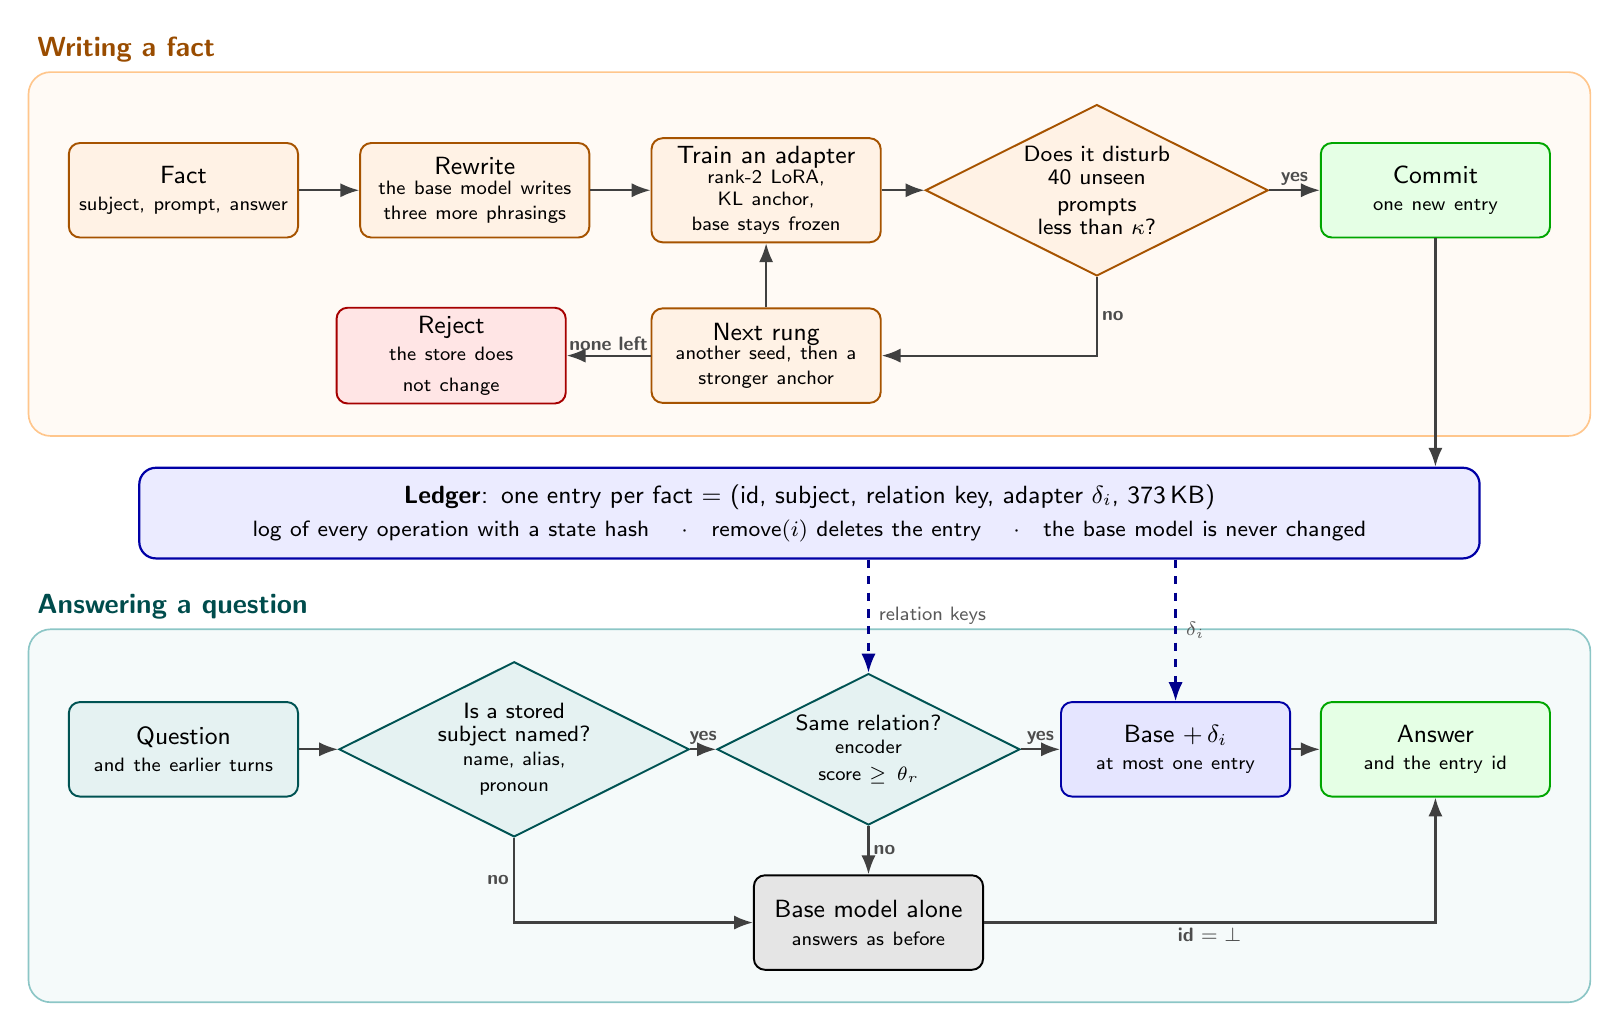
\begin{tikzpicture}[
  font=\sffamily\small,
  step/.style={draw=#1!65!black, fill=#1!10, rounded corners=4pt, align=center,
    minimum height=12mm, text width=27mm, inner sep=3pt, line width=0.7pt},
  step/.default=black,
  test/.style={draw=#1!65!black, fill=#1!10, diamond, aspect=2.0, align=center,
    inner sep=0pt, text width=21mm, font=\sffamily\footnotesize, line width=0.7pt},
  arr/.style={-{Latex[length=2.4mm,width=1.8mm]}, line width=0.8pt, draw=black!75},
  soft/.style={arr, dashed, draw=blue!55!black},
  lab/.style={font=\sffamily\scriptsize\bfseries, inner sep=1.5pt, text=black!70},
  sub/.style={font=\sffamily\scriptsize, text=black!65},
  lane/.style={draw=#1!45, fill=#1!4, rounded corners=8pt, line width=0.6pt},
  lanetitle/.style={font=\sffamily\bfseries, text=#1!60!black, anchor=south west},
]
% ---------------------------------------------------------------- write a fact
\node[step=orange] (fact) at (0,0) {Fact\\[-1pt]{\scriptsize subject, prompt, answer}};
\node[step=orange] (rew) at (3.7,0) {Rewrite\\[-1pt]{\scriptsize the base model writes\\[-2pt]three more phrasings}};
\node[step=orange] (train) at (7.4,0) {Train an adapter\\[-1pt]{\scriptsize rank-2 LoRA, KL anchor,\\[-2pt]base stays frozen}};
\node[test=orange] (gate) at (11.6,0) {Does it disturb\\[-1pt]40 unseen prompts\\[-1pt]less than $\kappa$?};
\node[step=green] (commit) at (15.9,0) {Commit\\[-1pt]{\scriptsize one new entry}};
\node[step=orange] (ladder) at (7.4,-2.1) {Next rung\\[-1pt]{\scriptsize another seed, then a\\[-2pt]stronger anchor}};
\node[step=red] (reject) at (3.4,-2.1) {Reject\\[-1pt]{\scriptsize the store does not change}};

\draw[arr] (fact) -- (rew);
\draw[arr] (rew) -- (train);
\draw[arr] (train) -- (gate);
\draw[arr] (gate) -- node[lab, above] {yes} (commit);
\draw[arr] (gate.south) |- node[lab, pos=0.25, right] {no} (ladder.east);
\draw[arr] (ladder) -- (train);
\draw[arr] (ladder) -- node[lab, above] {none left} (reject);

% ---------------------------------------------------------------- the ledger
\node[draw=blue!65!black, fill=blue!8, rounded corners=6pt, line width=0.8pt,
  text width=166mm, align=center, inner sep=6pt] (ledger) at (7.95,-4.1)
  {\textbf{Ledger}: one entry per fact $=$ (id, subject, relation key, adapter $\delta_i$, 373\,KB)\\[1pt]
   {\footnotesize log of every operation with a state hash \quad$\cdot$\quad
   remove$(i)$ deletes the entry \quad$\cdot$\quad the base model is never changed}};
\draw[arr] (commit.south) -- (commit.south |- ledger.north);

% ---------------------------------------------------------------- answer a question
\node[step=teal] (q) at (0,-7.1) {Question\\[-1pt]{\scriptsize and the earlier turns}};
\node[test=teal] (subj) at (4.2,-7.1) {Is a stored\\[-1pt]subject named?\\[-1pt]{\scriptsize name, alias, pronoun}};
\node[test=teal] (rel) at (8.7,-7.1) {Same relation?\\[-1pt]{\scriptsize encoder score $\ge\theta_r$}};
\node[step=blue] (adapt) at (12.6,-7.1) {Base $+\,\delta_i$\\[-1pt]{\scriptsize at most one entry}};
\node[step=green] (ans) at (15.9,-7.1) {Answer\\[-1pt]{\scriptsize and the entry id}};
\node[step=black] (base) at (8.7,-9.3) {Base model alone\\[-1pt]{\scriptsize answers as before}};

\draw[arr] (q) -- (subj);
\draw[arr] (subj) -- node[lab, above] {yes} (rel);
\draw[arr] (rel) -- node[lab, above] {yes} (adapt);
\draw[arr] (adapt) -- (ans);
\draw[arr] (subj.south) |- node[lab, pos=0.25, left] {no} (base.west);
\draw[arr] (rel) -- node[lab, right] {no} (base);
\draw[arr] (base.east) -| node[lab, pos=0.25, below] {id $=\bot$} (ans.south);
\draw[soft] (ledger.south -| rel.north) -- node[sub, right] {relation keys} (rel.north);
\draw[soft] (ledger.south -| adapt.north) -- node[sub, right] {$\delta_i$} (adapt.north);

% ---------------------------------------------------------------- lanes
\begin{scope}[on background layer]
  \node[lane=orange, fit=(fact)(commit)(gate)(reject)(ladder), inner xsep=5mm, inner ysep=4mm] (wl) {};
  \node[lane=teal, fit=(q)(ans)(subj)(base), inner xsep=5mm, inner ysep=4mm] (rl) {};
\end{scope}
\node[lanetitle=orange] at (wl.north west) {Writing a fact};
\node[lanetitle=teal] at (rl.north west) {Answering a question};
\end{tikzpicture}
}
\caption{Overview of RELIC's default store. Top: a fact is written by training a rank-2 adapter on
its edit prompt and on up to three rewrites by the base model, with a KL anchor on a copy of the frozen
base. The adapter is committed only if its divergence $D$ on 40 held-out prompts is at most $\kappa$;
otherwise the next rung of a ladder retrains it with another seed or a stronger anchor, and a fact
that passes no rung is rejected and changes nothing. Middle: the ledger holds one entry per fact and
logs every operation with a state hash; removal deletes the entry. Bottom: the router applies an
entry only if the question names a stored subject and asks for its relation; otherwise the base model
answers, and every answer carries the identifier of its entry.}
\label{fig:arch}
\end{figure*}


Fig.~\ref{fig:arch} shows the system and Algorithm~\ref{alg:txn} its operations. Table~\ref{tab:config}
in the appendix lists the configuration.

\subsection{Adapters}
An adapter is a LoRA update~\cite{hu2022lora} of rank 2 ($\alpha=4$) on the query and value projections
of all 28 layers, trained with LoRA+~\cite{hayou2024loraplus}: AdamW at a learning rate of
$3\cdot10^{-4}$ for $A$ and eight times that for $B$, 16 passes over the training pairs. The pairs are
the fact's statement mapped to an acknowledgment, the edit prompt mapped to the answer, and up to three
rewrites of the edit prompt mapped to the answer. The base model writes the rewrites from the subject
and the edit prompt alone, so no benchmark paraphrase enters training. The loss is
\begin{multline}
\mathcal{L}(\delta)=\sum_{(u,v)\in P(e)}\mathrm{CE}\big(v\mid u;\theta_0\oplus\delta\big)\\
+\frac{\lambda}{|Q|}\sum_{c\in Q}\mathrm{KL}\big(p_{\theta_0}(\cdot\mid c)\,\big\|\,
p_{\theta_0\oplus\delta}(\cdot\mid c)\big),
\label{eq:loss}
\end{multline}
with two generic anchor prompts $Q$ and $\lambda=1$ at the first attempt. The adapter is stored in int8
with one fp16 scale per row of $B$, 373\,KB per fact.

\subsection{Divergence Check}
\label{sec:checkmethod}
With $p_c=p_{\theta_0}(\cdot\mid c)$ and $\tilde p_c=p_{\theta_0\oplus\delta}(\cdot\mid c)$, a
candidate is scored by
\begin{equation}
D(\delta)=\frac{1}{|C|}\sum_{c\in C}\big[\mathrm{KL}(p_c\,\|\,\tilde p_c)
+\mathrm{KL}(\tilde p_c\,\|\,p_c)\big]
\end{equation}
on 40 canary prompts disjoint from $Q$ (factual questions, arithmetic, instructions and four other
languages), in its stored int8 form, and committed only if $D(\delta)\le\kappa$. The limit
$\kappa=\N{69:pooled:benign_r16:kappa}$ is the 99th percentile of $D$ over 100 adapters known to be
benign. The canaries must be held out from training: an adapter is trained to leave $Q$ unchanged, so
$D$ measured on $Q$ understates its footprint (Section~\ref{sec:check}).

\subsection{Retry Ladder}
\label{sec:ladder}
A candidate above $\kappa$ is not discarded at once. The write tries a ladder of retrainings and stores
the first one under $\kappa$: the same recipe with another seed, then anchor weights
$\lambda\in\{2,4,8,16\}$, then the recipe without rewrites. If no rung passes, the write commits
nothing. The choice of rung reads only $D$, never a paraphrase.

\subsection{Router}
\label{sec:router}
The router has no parameters trained on the stored facts and works in three steps.
\begin{enumerate}
\item Entity match. Query and stored subjects are normalized, and a subject or one of its aliases
matches if it occurs on word boundaries, or if each of its tokens matches a consecutive query token,
exactly for tokens under four characters and within an edit distance of 1 (2 from six characters)
otherwise. The entries whose subject is the longest match are the candidates; with none, the router
returns $\bot$. A pronoun is resolved from the conversation when an earlier turn spells out a stored
subject.
\item Clause. Only the sentence of the query that contains the subject is kept.
\item Relation. The subject is masked in this clause and in each candidate's edit prompt, a relation
encoder embeds both, and the most similar candidate is selected if the cosine similarity reaches a
threshold.
\end{enumerate}
The relation encoder is all-mpnet-base-v2~\cite{song2020mpnet,reimers2019sbert} trained once, offline,
on 7500 triplets of relation templates (anchor and positive from one relation, negative from another)
from 3000 CounterFact and 1500 zsRE facts that share no subject with any evaluation set; 11 of the 34
CounterFact relations are held out from it. The global threshold $\tau=0.7501$ is the lowest that routes
at most 5\% of other-relation queries on a disjoint development split. Where an entry carries a relation
identifier, a stricter per-relation threshold $\tau_r$ applies to nine relations whose neighboring
questions were frequently routed in a calibration set disjoint from the test facts.

\subsection{Writes, Removal and Logging}
A write first looks for an entry with the same subject whose relation text scores above $\tau$. If it
holds the same answer, the write joins it as another phrasing, since a query would reach that entry
anyway. If it holds another answer, the write replaces it only above a stricter threshold of $0.8985$,
since a replacement drops a fact. \revoke$(i)$ deletes entry $i$ and its phrasings. For serving, the
selected adapter is written into a LoRA slot and all other slots are zero. The log records the
identifier, the rung, $D$, the training time and the state hash. Commits from threads of one process are
serial under a lock and the store file is replaced atomically; processes are not isolated from each
other, so a transaction here is the single-writer operation of Proposition~\ref{prop:atomic}.

\begin{algorithm}[t]
\caption{Operations on the store}
\label{alg:txn}
\begin{algorithmic}[1]
\Function{Add}{$e$, $i$}
  \If{an entry of the same subject and relation holds $a_e$} \State add $x_e$ as a phrasing; log and \Return \EndIf
  \State $W\gets$ rewrites of $x_e$ by $f_{\theta_0}$
  \For{each rung (seed, $\lambda$, rewrites or none) of the ladder}
    \State $\delta\gets\arg\min\mathcal{L}$ on a copy of $\theta_0$ \Comment{Eq.~\eqref{eq:loss}}
    \If{$D(\delta)\le\kappa$}
      \State $S\gets S\cup\{(i,\delta,k_e,s_e,r_e)\}$; log$(\textsc{add},i,h(S))$; \Return
    \EndIf
  \EndFor
  \State log$(\textsc{reject},i)$ \Comment{$S$ unchanged}
\EndFunction
\Function{Serve}{$q$}
  \State $j\gets\rho_S(q)$; \Return $\big(f_{\theta_0\oplus\delta_j}(q),\ j\big)$ \Comment{$j=\bot$: base}
\EndFunction
\Function{Remove}{$i$}
  \State $S\gets S\setminus\{i\}$; log$(\textsc{remove},i,h(S))$
\EndFunction
\end{algorithmic}
\end{algorithm}

% ===========================================================================
\section{Experimental Setup}
\label{sec:setup}

\subsection{Model and Facts}
The base model is Qwen2.5-1.5B-Instruct~\cite{qwen2024qwen25} in bf16 on one shared 8\,GB GPU, served
with its chat template, the system prompt ``Answer briefly.'', greedy decoding and at most 64 new
tokens. Facts come from the ROME versions of CounterFact~\cite{meng2022rome} and
zsRE~\cite{levy2017zeroshot,decao2021editing}. CounterFact targets are counterfactual, so the base model
does not produce them; zsRE uses the reference answer, which the base model often knows. Two sets are
used. The main stores hold 1000 facts per dataset and were read by many decisions over the course of the
work. The fresh set holds 400 facts per dataset drawn with a new seed, disjoint by subject from the main
stores, the development split and every earlier draw, and was read once, for the comparison of
Section~\ref{sec:fresh}.

\subsection{Queries}
Each fact has an edit prompt and a held-out paraphrase. Queries that should not use a stored fact are of
four kinds. E3 prompts ask about a stored subject with the template of another CounterFact relation. E2
prompts ask the stored relation about another subject. Natural questions about another relation of a
stored subject are written by SmolLM3-3B, half about a neighboring relation (the language a person
speaks, when the stored fact is the native language) and half about a uniformly drawn one. Synthetic
distractors and zsRE locality questions name no stored subject. A wrong route is read on 1000 zsRE
development questions whose base answer is correct, each answered with an unrelated entry forced.
General capability is read on 500 MMLU~\cite{hendrycks2021mmlu} and 500
ARC-Challenge~\cite{clark2018arc} questions.

\subsection{Metrics}
The metrics are fixed in entry 157 of the record. A response is correct if it contains the target at a
word boundary. Edit accuracy is the share of correct responses to edit prompts and paraphrase accuracy
the share for held-out paraphrases, both routed. A response leaks if it contains a stored target that
the base model's response to the same query does not; the leak rate is reported separately for E3, E2 and
natural questions. Wrong-route retention is the share of base-correct answers kept with an entry forced.
Removal is read on 100 removed facts as return (correct exactly when the base model is correct) and on
the others as retention of edit accuracy. Capability cost is MMLU and ARC accuracy with a random entry
forced, minus the base model's. Intervals are 95\% bootstrap intervals over facts or questions;
comparisons are paired, and a non-inferiority margin is read against the lower end of the one-sided
95\% interval.

\subsection{Pre-Registration}
Each run was entered in the record with its arms, metrics, predictions and decision rule before it
started, and tagged in git. Failed predictions and failed rules are reported as such, deviations are
written down with their reason, and a result read after a decision is labelled as read after it. We refer
to an entry by E and its number, for example E137.

% ===========================================================================
\section{Results}
\label{sec:results}

\subsection{The Store on Fresh Facts}
\label{sec:fresh}

\begin{table}[t]
\centering
\caption{The store on 800 fresh facts (400 per dataset), served through the router (\entry{137},
\entry{139}). Default: adapter alone, global threshold; $+\tau_r$: with per-relation thresholds; with
note: the earlier store, which served each adapter with the fact's statement in the system prompt;
first recipe: the adapter without rewrites, served alone.}
\label{tab:fresh}
\scriptsize
\setlength{\tabcolsep}{3.5pt}
\begin{tabular}{lcccc}
\toprule
 & Default & $+\tau_r$ & With note & First recipe \\
\midrule
Edit accuracy, CounterFact & \N{137:counterfact:default:edit_accuracy} & \N{139:counterfact:default:edit_accuracy_relation_tau} & \N{137:counterfact:adapter_and_note:edit_accuracy} & \N{137:counterfact:A0_alone:edit_accuracy} \\
Paraphrase accuracy, CounterFact & \N{137:counterfact:default:paraphrase_accuracy} & \N{139:counterfact:default:paraphrase_accuracy} & \N{137:counterfact:adapter_and_note:paraphrase_accuracy} & \N{137:counterfact:A0_alone:paraphrase_accuracy} \\
Paraphrase accuracy, zsRE & \N{137:zsre:default:paraphrase_accuracy} & \N{139:zsre:default:paraphrase_accuracy_relation_tau} & \N{137:zsre:adapter_and_note:paraphrase_accuracy} & \N{137:zsre:A0_alone:paraphrase_accuracy} \\
Leak rate, E3 & \N{137:counterfact:default:leak_rate_e3} & \N{139:counterfact:default:leak_rate_e3_relation_tau} & \N{137:counterfact:adapter_and_note:leak_rate_e3} & \N{137:counterfact:A0_alone:leak_rate_e3} \\
Leak rate, natural, all & \N{137:counterfact:default:leak_rate_natural} & \N{139:counterfact:default:leak_rate_natural_relation_tau} & \N{137:counterfact:adapter_and_note:leak_rate_natural} & \N{137:counterfact:A0_alone:leak_rate_natural} \\
Leak rate, natural, neighboring & \N{137:counterfact:default:leak_rate_natural_near} & \N{139:counterfact:default:leak_rate_natural_near} & \N{137:counterfact:adapter_and_note:leak_rate_natural_near} & \N{137:counterfact:A0_alone:leak_rate_natural_near} \\
Leak rate, natural, uniform & \N{137:counterfact:default:leak_rate_natural_uniform} & \N{139:counterfact:default:leak_rate_natural_uniform_relation_tau} & \N{137:counterfact:adapter_and_note:leak_rate_natural_uniform} & -- \\
\bottomrule
\end{tabular}
\end{table}

Until \entry{143}, RELIC stored a note with each fact, its statement placed in the system prompt, and
served it together with the adapter. A store with no note is simpler, puts no stored text into the
prompt and, as Section~\ref{sec:wrong} shows, damages less when it is routed wrongly. The registered
question was whether it loses answers. On the fresh set, against the store with note, its paraphrase
accuracy differs by \N{137:pooled:default_minus_adapter_and_note:diff_paraphrase_accuracy} pooled and by
\N{137:counterfact:default_minus_adapter_and_note:diff_paraphrase_accuracy}
\CI{137:counterfact:default_minus_adapter_and_note:diff_paraphrase_accuracy} on CounterFact
(Table~\ref{tab:fresh}). The rule required the lower end of the one-sided interval to stay above
$-0.03$; on CounterFact it was
\N{137:counterfact:default_minus_adapter_and_note:diff_paraphrase_accuracy_lower_one_sided}, so the rule
failed and a loss of that size is not excluded. Edit accuracy is higher without the note,
\N{137:pooled:default_minus_adapter_and_note:diff_edit_accuracy}
\CI{137:pooled:default_minus_adapter_and_note:diff_edit_accuracy} pooled, and the leak rates do not
separate the two stores (E3 \N{137:counterfact:default_minus_adapter_and_note:diff_leak_rate_e3},
natural \N{137:counterfact:default_minus_adapter_and_note:diff_leak_rate_natural}). The author then made
the store with no note the default (\entry{143}); it is reported here as having failed its rule.

The rewrites carry the gain over the first recipe: paraphrase accuracy rises by
\N{137:pooled:default_minus_A0_alone:diff_paraphrase_accuracy} pooled. The remaining gap to the store
with note lies on facts that pass the check at the first attempt, not on those the check rejects: the
store matches the paraphrase accuracy of a store that keeps every first attempt regardless of the check
(\N{137:pooled:gate_off:paraphrase_accuracy} against \N{137:pooled:default:paraphrase_accuracy}). No edit
or paraphrase query was routed to another fact's entry, and the store holds
\Pct{137:pooled:default:facts_with_entry}\% of the facts.

\subsection{The Store on the Main CounterFact Store}
\label{sec:seen}

\begin{table}[t]
\centering
\caption{The 1000 facts of the main CounterFact store, written through the library's own write path
(\entry{146}). Paired readings cut responses to 24 tokens, the length of the saved readings of the store
with note.}
\label{tab:seen}
\scriptsize
\begin{tabular}{lcc}
\toprule
 & Default & With note \\
\midrule
Edit accuracy & \N{146:counterfact:default:edit_accuracy} & \N{146:counterfact:adapter_and_note_r2:edit_accuracy} \\
Paraphrase accuracy & \N{146:counterfact:default:paraphrase_accuracy} & \N{146:counterfact:adapter_and_note_r2:paraphrase_accuracy} \\
Leak rate, E3, with $\tau_r$ & \N{146:counterfact:default:leak_rate_e3} & \N{146:counterfact:adapter_and_note_r2:leak_rate_e3} \\
Leak rate, E2 & \N{146:counterfact:default:leak_rate_e2} & \N{146:counterfact:adapter_and_note_r2:leak_rate_e2} \\
Leak rate, natural, neighboring, with $\tau_r$ & \N{146:counterfact:default:leak_rate_natural_near_relation_tau} & -- \\
Removal: return to base (100 removed) & \N{146:counterfact:default:removal_return} & \N{146:counterfact:adapter_and_note_r2:removal_return} \\
Removal: retention of the others & \N{146:counterfact:default:retention} & \N{146:counterfact:adapter_and_note_r2:retention} \\
Wrong-route retention (998 questions) & \N{146:counterfact:default:wrong_route_retention} & \N{146:counterfact:adapter_and_note_r2:wrong_route_retention} \\
Capability cost, entry forced & \N{146:mmlu_arc:default:capability_cost} & \N{146:mmlu_arc:adapter_and_note_r2:capability_cost} \\
\bottomrule
\end{tabular}
\end{table}

The main CounterFact store was rebuilt with the default write path, one fact after another, so that
same-answer writes join existing entries as they would in use (Table~\ref{tab:seen}). These facts had
been read before, so this is a comparison with the earlier tables and not a confirmation. Here the note
is worth more: paraphrase accuracy differs by
\N{146:counterfact:default_minus_adapter_and_note_r2:diff_paraphrase_accuracy}
\CI{146:counterfact:default_minus_adapter_and_note_r2:diff_paraphrase_accuracy}, twice the gap on fresh
facts. Every removed fact returns to the base answer in both stores, the other facts keep their answers,
and none of 1000 MMLU and ARC questions is routed in either. The zsRE half of this evaluation stopped
after 550 of 1000 writes and has not been read.

\subsection{Divergence Check}
\label{sec:check}
An adapter trained with the KL anchor of Eq.~\eqref{eq:loss} keeps the anchor prompts almost unchanged,
so $D$ on them is small for every adapter: a mean of \N{69:pooled:benign_r16:d_train_mean} over 100
benign adapters, against \N{69:pooled:benign_r16:d_heldout_mean} on the 40 held-out canaries
(\entry{69}). Ten adapters trained without the anchor and at a high learning rate, meant to be harmful,
exceed both the old in-sample limit and $\kappa$, but the in-sample margin is nil, while on held-out
canaries the closest harmful adapter scores \N{69:pooled:harmful:d_heldout_min}, more than three times
$\kappa$. The check on held-out prompts is therefore the one the system uses.

\subsection{The Write Path and Its Cost}
\label{sec:write}
On the fresh set \Pct{137:pooled:default:first_attempt_reject_share}\% of first attempts exceed $\kappa$,
and on the main CounterFact store \Pct{146:counterfact:default:first_attempt_reject_share}\% do. The ladder
recovers almost all of them: \Pct{146:counterfact:default:no_entry_share}\% of the main-store facts end
with no entry. Part of what the check rejects is the training draw and not the fact: on a development set
of 19 rejected facts, \N{135:pooled:new_seed:rejected_under_kappa} came under $\kappa$ with one of two
new seeds (\entry{135}). A write took \N{146:counterfact:default:seconds_per_write_median}\,s at the median
on a GPU shared with other work, a removal \N{146:counterfact:default:seconds_per_removal}\,s, and each
fact stores 373\,KB. In the earlier store with notes, only the facts whose note failed received an
adapter; in the default store every fact does.

\subsection{The Cost of a Wrong Route}
\label{sec:wrong}

\begin{table}[t]
\centering
\caption{Wrong-route retention: share of base-correct zsRE questions still answered correctly with an
unrelated entry forced (1000 questions, \entry{114}; 998 for the default store, \entry{146}), and
capability cost on 500 MMLU and 500 ARC questions with a random entry forced (\entry{116},
\entry{146}).}
\label{tab:wrong}
\scriptsize
\begin{tabular}{lcc}
\toprule
Entry served & Retention & Capability cost \\
\midrule
Adapter, rank 16 & \N{114:zsre_dev:adapter_r16:wrong_route_retention} & \N{116:mmlu_arc:adapter_r16:capability_cost} \\
Adapter, rank 2 & \N{114:zsre_dev:adapter_r2:wrong_route_retention} & \N{116:mmlu_arc:adapter_r2:capability_cost} \\
Note alone & \N{114:zsre_dev:note:wrong_route_retention} & \N{116:mmlu_arc:note:capability_cost} \\
Adapter and note, rank 2 & \N{114:zsre_dev:adapter_and_note_r2:wrong_route_retention} & \N{146:mmlu_arc:adapter_and_note_r2:capability_cost} \\
Default store (adapter with rewrites) & \N{146:counterfact:default:wrong_route_retention} & \N{146:mmlu_arc:default:capability_cost} \\
\bottomrule
\end{tabular}
\end{table}

A wrong route is the failure that costs most per query (Table~\ref{tab:wrong}). An entry forced onto an
unrelated question keeps between a third and two thirds of the base model's correct answers, and the
note does more damage than the adapter: the combination with note keeps
\N{114:zsre_dev:adapter_and_note_r2:wrong_route_retention}, and the default store keeps
\N{146:counterfact:default_minus_adapter_and_note_r2:diff_wrong_route_retention} more on the same
questions. The adapter trained on rewrites keeps less than the first recipe's adapter, which saw only the
edit prompt. The router's false-route rate is what keeps this cost small: none of the 1000 MMLU and ARC
questions is routed, so served accuracy equals the base model's \N{116:mmlu_arc:base:accuracy}, and the
cost in Table~\ref{tab:wrong} applies only to the routed share. Forcing an entry onto a multiple-choice
question costs about 2 points at most, far less than on short factual answers, the form the adapters are
trained on.

\subsection{Removal and Repeated Writes}
Removal is exact by Proposition~\ref{prop:identity}, and on the CounterFact stores every removed fact
returns to the base answer. On zsRE an earlier per-entry store returned only
\N{122:zsre:per_entry:removal_return}, because one fact was often written several times and a removal
deleted one copy. Since same-answer writes join one entry, return is
\N{122:zsre:asymmetric_slots:removal_return} on the main zsRE store (\entry{122}), and on 1000 fresh zsRE
records with repeated subjects the share of removed facts still routed somewhere falls from
\N{115:zsre:per_entry:residual_route_share} to \N{115:zsre:asymmetric_slots:residual_route_share}
(\entry{115}). No write merged two different answers.

\subsection{Routing and Leakage}
\label{sec:leak}
The trained relation encoder replaced a general-purpose one because it routes paraphrases far better:
\N{76:counterfact:relenc:paraphrase_route_correct} of CounterFact paraphrases reach their entry, against
\N{76:counterfact:minilm:paraphrase_route_correct} (\entry{76}). The gain is uneven. On relations seen in
its training it routes \N{76:counterfact:relenc:paraphrase_route_correct_seen_relations} of paraphrases,
on the 11 held-out relations \N{76:counterfact:relenc:paraphrase_route_correct_heldout_relations}, and on
held-out relations its leakage does not fall. Its success is therefore a statement about a deployment whose
relation inventory is known in advance.

The leak that remains comes from neighboring relations. Template prompts about another relation leak in
\Pct{137:counterfact:default:leak_rate_e3}\% of cases, because CounterFact pairs relations uniformly.
Natural questions about a neighboring relation of a stored subject leak far more:
\Pct{137:counterfact:default:leak_rate_natural_near}\% on fresh facts with the global threshold.
Per-relation thresholds lower this to \Pct{139:counterfact:default:leak_rate_natural_near}\% at a quarter
of a point of paraphrase accuracy (\entry{139}); a stricter recipe reached
\Pct{139:counterfact:default:leak_rate_natural_near_rall}\% and failed its paraphrase margin. The router's
score separates paraphrases from these questions well (AUROC
\N{139:counterfact:router_score:auroc_paraphrase_vs_near}), so the leak lies where the threshold is placed
rather than in a score that cannot tell the two apart.

Not every such leak is wrong. When the stored fact is that a film's original language is French, the
stored answer is also correct for the question of which language the film is in. The author labelled 200
sampled items as correct, leak or unsure. On items where neither the author nor a model labeler was
unsure, the two agree with Cohen's~\cite{cohen1960kappa}
$\kappa=\N{140:counterfact:author_vs_model:cohen_kappa_two_class}$
\CI{140:counterfact:author_vs_model:cohen_kappa_two_class}, and the corrected neighboring-relation leak of
the router is \N{140:counterfact:default_router:leak_rate_natural_near_corrected}, on 27 items
(\entry{140}). The per-relation thresholds remove labelled correct answers and labelled leaks at similar
rates, \N{142:counterfact:R107:legit_removed_share} and \N{142:counterfact:R107:leak_removed_share}
(\entry{142}), so the fall in the automatic count is not all gain. A frozen entailment model,
DeBERTa-v3-large trained on NLI~\cite{he2023debertav3}, that reads the stored fact and the question ranks
correct answers above leaks better than the router's score (AUROC
\N{148:counterfact:nli_entailment:auroc_legit_vs_leak} against
\N{148:counterfact:router_score:auroc_legit_vs_leak}), but at a threshold that keeps 90\% of correct
answers it removes too few leaks, and it failed its rule (\entry{148}).

\subsection{Another Language}
\label{sec:lang}

\begin{table}[t]
\centering
\caption{Router AUROC on 1031 BMIKE-53 CounterFact facts: a query about the stored fact against a query
about another relation of the same subject (\entry{156}, \entry{159}). The store holds English entries.}
\label{tab:lang}
\scriptsize
\begin{tabular}{lcc}
\toprule
Relation encoder & English & Turkish \\
\midrule
all-mpnet-base-v2, untrained & \N{156:bmike_en:mpnet:router_auroc} & \N{156:bmike_tr:mpnet:router_auroc} \\
Trained (default) & \N{156:bmike_en:relenc:router_auroc} & \N{156:bmike_tr:relenc:router_auroc} \\
Multilingual mpnet, untrained & \N{156:bmike_en:mmpnet:router_auroc} & \N{156:bmike_tr:mmpnet:router_auroc} \\
Multilingual mpnet, trained & \N{156:bmike_en:relenc-m:router_auroc} & \N{156:bmike_tr:relenc-m:router_auroc} \\
\quad with translated triplets & \N{159:bmike_en:relenc-b:router_auroc} & \N{159:bmike_tr:relenc-b:router_auroc} \\
\bottomrule
\end{tabular}
\end{table}

BMIKE-53 provides CounterFact facts with questions in other languages~\cite{nie2025bmike}. With English
entries and Turkish questions, the default router is at chance (Table~\ref{tab:lang}) and sends
\Pct{156:bmike_tr:relenc:src_routed_right}\% of Turkish questions to their entry, so in Turkish the common
failure is the lost fact rather than the leak. Training the same triplets on a multilingual base,
paraphrase-multilingual-mpnet-base-v2~\cite{reimers2020multilingual}, repairs Turkish and costs some
English AUROC; the registered margin of $-0.02$ on English was missed by 0.0001. Adding triplets
translated by OPUS-MT~\cite{tiedemann2020opusmt} lowered both languages (\entry{159}). The English gap is
already present in the untrained multilingual base. A second finding concerns English: BMIKE-53
rephrasings are questions, and at the operating point the router sends only
\Pct{156:bmike_en:relenc:rephrase_routed_right}\% of them to their entry, since the stored keys are cloze
prompts.

\subsection{Other Base Models}
\label{sec:scale}

\begin{table}[t]
\centering
\caption{The earlier store with notes on five base models, 2000 facts (\entry{120}). Need: share of facts
whose note does not answer the edit prompt, so that they receive an adapter. Paraphrase: accuracy of that
store. Above $\kappa$: share of CounterFact adapters over the limit calibrated on Qwen2.5-1.5B.}
\label{tab:scale}
\scriptsize
\setlength{\tabcolsep}{3pt}
\begin{tabular}{lcccc}
\toprule
Model & Need (\%) & \multicolumn{2}{c}{Paraphrase} & Above $\kappa$ \\
 & & CF & zsRE & \\
\midrule
Qwen2.5-0.5B & \Pct{120:pooled:qwen2.5-0.5b:need_adapter_share} & \N{120:counterfact:qwen2.5-0.5b:tiered_paraphrase_accuracy} & \N{120:zsre:qwen2.5-0.5b:tiered_paraphrase_accuracy} & \N{120:counterfact:qwen2.5-0.5b:above_kappa_share} \\
Qwen2.5-1.5B & \Pct{120:pooled:qwen2.5-1.5b:need_adapter_share} & \N{120:counterfact:qwen2.5-1.5b:tiered_paraphrase_accuracy} & \N{120:zsre:qwen2.5-1.5b:tiered_paraphrase_accuracy} & \N{120:counterfact:qwen2.5-1.5b:above_kappa_share} \\
Qwen2.5-1.5B, 4-bit & \Pct{120:pooled:qwen2.5-1.5b-4bit:need_adapter_share} & \N{120:counterfact:qwen2.5-1.5b-4bit:tiered_paraphrase_accuracy} & \N{120:zsre:qwen2.5-1.5b-4bit:tiered_paraphrase_accuracy} & \N{120:counterfact:qwen2.5-1.5b-4bit:above_kappa_share} \\
Qwen2.5-3B, 4-bit & \Pct{120:pooled:qwen2.5-3b-4bit:need_adapter_share} & \N{120:counterfact:qwen2.5-3b-4bit:tiered_paraphrase_accuracy} & \N{120:zsre:qwen2.5-3b-4bit:tiered_paraphrase_accuracy} & \N{120:counterfact:qwen2.5-3b-4bit:above_kappa_share} \\
Qwen2.5-7B, 4-bit & \Pct{120:pooled:qwen2.5-7b-4bit:need_adapter_share} & \N{120:counterfact:qwen2.5-7b-4bit:tiered_paraphrase_accuracy} & \N{120:zsre:qwen2.5-7b-4bit:tiered_paraphrase_accuracy} & \N{120:counterfact:qwen2.5-7b-4bit:above_kappa_share} \\
SmolLM3-3B, 4-bit & \Pct{120:pooled:smollm3-3b-4bit:need_adapter_share} & \N{120:counterfact:smollm3-3b-4bit:tiered_paraphrase_accuracy} & \N{120:zsre:smollm3-3b-4bit:tiered_paraphrase_accuracy} & \N{120:counterfact:smollm3-3b-4bit:above_kappa_share} \\
\bottomrule
\end{tabular}
\end{table}

The store with no note has been run on Qwen2.5-1.5B only. What other base models can tell comes from the
earlier store with notes, where a fact received an adapter only if its note failed
(Table~\ref{tab:scale}). The share of such facts does not follow model size: it is lowest at 0.5B,
\Pct{120:pooled:qwen2.5-0.5b:need_adapter_share}\%, highest at 1.5B,
\Pct{120:pooled:qwen2.5-1.5b:need_adapter_share}\%, and SmolLM3-3B needs half of what the Qwen model of that size needs. The two 1.5B arms show that
4-bit quantization does not explain the differences. The divergence limit does not transfer: calibrated on
1.5B, it rejects most adapters of the 3B and 7B models. Whether those adapters are harmful is not measured,
and the default store, in which every fact receives an adapter, cannot be used on those models until
$\kappa$ is calibrated for each.

\subsection{Alternatives That Failed Their Rules}
\label{sec:alt}

\begin{table}[t]
\centering
\caption{Alternatives to the trained per-fact adapter, each with its registered decision rule; none was
adopted. Readings are forced, with the right entry applied.}
\label{tab:alt}
\scriptsize
\setlength{\tabcolsep}{2.5pt}
\begin{tabular}{>{\raggedright\arraybackslash}p{2.2cm}>{\raggedright\arraybackslash}p{5.8cm}}
\toprule
Alternative & Reading \\
\midrule
Soft prompt (\entry{128}) & edit accuracy \N{128:pooled:soft_prompt:edit_accuracy} and paraphrase \N{128:pooled:soft_prompt:paraphrase_accuracy}, against \N{89:pooled:rank2_int8:edit_accuracy} and \N{89:pooled:rank2_int8:paraphrase_accuracy} for the adapter \\
LoReFT, DiReFT (\entry{93}) & most interventions above $\kappa$; \N{93:pooled:direft_r4:above_kappa_share} for the best variant \\
Shared by 8 to 32 facts (\entry{124}) & paraphrase with note \N{124:counterfact:shard_8x2:paraphrase_accuracy} at best, against \N{124:counterfact:per_fact_r2:paraphrase_accuracy} per fact \\
Hypernetwork (\entry{150}) & edit accuracy \N{150:counterfact:hypernet_H1000:unseen_edit_accuracy} on unseen facts, \N{150:counterfact:hypernet_H1000:train_edit_accuracy} on training facts \\
Hypernetwork given the answer (\entry{152}) & \N{152:counterfact:hypernet_H0_Eb:unseen_edit_accuracy} on unseen facts; no adapter under $\kappa$ \\
Null space, 90\% (\entry{155}) & wrong-route retention \N{155:counterfact:nullspace_N90:wrong_route_retention} against \N{155:counterfact:trained_T:wrong_route_retention}; paraphrase \N{155:counterfact:nullspace_N90:paraphrase_accuracy} against \N{155:counterfact:trained_T:paraphrase_accuracy} \\
Hard negatives (\entry{123}) & neighboring questions routed \N{123:counterfact:hardB:natural_near_routed} against \N{123:counterfact:baseline:natural_near_routed} \\
\bottomrule
\end{tabular}
\end{table}

Table~\ref{tab:alt} lists the alternatives. Two were aimed at storage and write time. A hypernetwork that
reads a fact and writes its rank-2 adapter in one forward pass costs milliseconds per adapter instead of
seconds and fits its 1000 training facts, but answered one unseen edit prompt in ten. Given the answer's
identity as input it answered \N{152:counterfact:hypernet_H0_Eb:unseen_edit_accuracy}, short of the
threshold of 1.00 that the author set for continuing, and none of its adapters stayed under $\kappa$, so
the line closed (\entry{152}). Projecting each adapter's input away from the directions that carry 90\% of
the energy of ordinary prompts, the idea of AlphaEdit~\cite{fang2025alphaedit}, kept more correct answers
under a wrong route and cut the median divergence tenfold, but lost most paraphrases. At this granularity
locality and generalization draw on the same directions (\entry{155}).

\subsection{Comparison with Editing Methods}

\begin{table}[t]
\centering
\caption{Edit accuracy on CounterFact under the chat template, substring score. Descriptive only, as the
sets differ in size and RELIC is shown in its earlier form with note (\entry{37}, \entry{54},
\entry{63}).}
\label{tab:baselines}
\scriptsize
\begin{tabular}{lcc}
\toprule
Method & Facts & Edit accuracy \\
\midrule
Instructed retrieval of the statement & 1000 & \N{37:counterfact:rag_instruct:edit_accuracy} \\
GRACE, official implementation & 200 & \N{54:counterfact:grace_easyedit:edit_accuracy} \\
WISE, official implementation & 200 & \N{54:counterfact:wise_easyedit:edit_accuracy} \\
WISE with its merge after 200 edits & 200 & \N{63:counterfact:wise_easyedit_merge200:edit_accuracy} \\
RELIC, rank 16 with note & 1000 & \N{37:counterfact:adapter_and_note_r16:edit_accuracy} \\
\bottomrule
\end{tabular}
\end{table}

Table~\ref{tab:baselines} compares RELIC with retrieval and with GRACE and WISE, run through
EasyEdit~\cite{wang2024easyedit} as 200 sequential edits. The comparison is descriptive and depends on
the prompt format. GRACE answers every edit on the plain edit prompt and few under the chat template,
because its keys are activations of the plain prompt's last token. WISE answers each edit right after it
is made, but after 200 sequential edits the final model answers few of them. Neither offers an operation
that removes one edit.

% ===========================================================================
\section{Discussion}
\label{sec:discussion}

\subsection{What the Measurements Show}
A per-fact adapter behind a router does what the data structure promises: removal returns the base answer,
the state hash returns to its earlier value, and the router leaves benchmark questions alone. The weak
points lie elsewhere. The first is the boundary between neighboring relations, where about one neighboring
question in six still receives the stored answer and about half of those answers are correct. None of the
text signals we tried, thresholds, mined negatives or an entailment model, tells the two kinds apart,
since whether the stored answer is right depends on what the asked relation means for that subject. The
second is the cost of an error: a wrong route damages almost half of the answers it touches, so routing
precision is a safety property and not only an accuracy one. The third is coverage. The router reads cloze
prompts better than questions and English better than Turkish. A multilingual encoder recovers Turkish at a
small cost in English, which a router that chooses its encoder by the language of the query would avoid by
construction; that design has not been registered or run.

Dropping the note made the system simpler and a wrong route cheaper, at a cost on CounterFact paraphrases
that the registered margin could not exclude. We report the decision as the author's and the rule as
failed. Every fact now receives an adapter of 373\,KB and, on our shared GPU, about 20 seconds of training.
The two alternatives that would have lowered that cost, a hypernetwork and adapters shared by several
facts, failed their rules.

\subsection{Limitations}
All default-store readings are on Qwen2.5-1.5B-Instruct, and the divergence limit must be calibrated on each
base model before the store is used there. Facts have single-token targets from two benchmarks, and no
multi-hop or reverse question was tested. The zsRE half of the main default-store evaluation is unfinished.
The natural questions were written by one model, the corrected leak rests on 27 labelled items, and pronoun
handling was tested on constructed conversations. Time to first token is part of the registered cost
metrics and has not been measured. The state hash names the model without its revision. A transaction is
atomic for one writer; two processes writing one store are not coordinated.

% ===========================================================================
\section{Conclusion}
RELIC stores each fact as its own rank-2 adapter behind a router whose parameters do not depend on the
stored facts, so that removal and attribution are exact by construction. In a pre-registered study the store
answers almost all edit prompts and most paraphrases on facts no decision had seen, leaves benchmark
questions untouched and returns removed facts to the base answer. It leaks into neighboring relations, does
not read a second language, and loses about half of the answers a wrong route touches. Several ways to make
it cheaper or more local failed their rules, and they are reported with the same weight as the results that
held. The record, the code and the tables behind every number are public.

% ===========================================================================
\appendix

\begin{table}[h]
\centering
\caption{Configuration of the default store.}
\label{tab:config}
\scriptsize
\resizebox{\columnwidth}{!}{%
\begin{tabular}{ll}
\toprule
Base model & Qwen2.5-1.5B-Instruct, bf16, frozen \\
Adapter & LoRA $r{=}2$, $\alpha{=}4$, query and value projections, 28 layers \\
Optimizer & AdamW, lr $3{\cdot}10^{-4}$ ($A$), $2.4{\cdot}10^{-3}$ ($B$, LoRA+), 16 passes \\
Training pairs & statement, edit prompt and up to 3 rewrites by the base model \\
Anchor & forward KL to the base on 2 generic prompts, $\lambda{=}1$ \\
Storage & int8 with an fp16 scale per row of $B$, 373\,KB \\
Divergence check & Jeffreys divergence on 40 held-out canaries, $\kappa{=}\N{69:pooled:benign_r16:kappa}$ \\
Retry ladder & another seed; $\lambda\in\{2,4,8,16\}$; no rewrites; else reject \\
Relation encoder & all-mpnet-base-v2, 7500 triplets, MNRL, lr $2{\cdot}10^{-5}$, one epoch \\
Thresholds & $\tau{=}0.7501$; per-relation for 9 relations; replacement at 0.8985 \\
Entity match & word boundary, or edit distance $\le 1$ (4+ characters), $\le 2$ (6+) \\
Serving & chat template, ``Answer briefly.'', greedy, 64 new tokens \\
Scoring & target at a word boundary \\
\bottomrule
\end{tabular}}
\end{table}

\bibliographystyle{IEEEtran}
\bibliography{IEEEctl,refs}

\end{document}
